% !Mode:: "TeX:UTF-8"
%!TEX program  = xelatex

%\documentclass[bwprint,fontset=windows]{gmcmthesis}
\documentclass[bwprint]{gmcmthesis}

\hypersetup{hidelinks}
\usepackage[framemethod=TikZ]{mdframed}

%\usepackage{fontspec}  % for Consolas & Courier New
%\lstset{basicstyle=\small\fontspec{Consolas}}
%\lstset{basicstyle=\small\fontspec{Courier New}}
%\setmonofont{Consolas}
%\setcounter{tocdepth}{3}   % 调整目录深度

\usepackage{subfig}
\usepackage{siunitx}

\usepackage{colortbl}
\definecolor{color1}{rgb}{0.78,0.88,0.99}
\definecolor{color2}{rgb}{0.36,0.62,0.84}
%\definecolor{color3}{rgb}{0.8235,0.8706,0.9373}
\definecolor{color3}{rgb}{0.88,0.92,0.96}
\definecolor{color4}{rgb}{0.96,0.97,0.98}%{0.9176,0.9373,0.9686}

% 算法
\usepackage[noend]{algpseudocode}
\usepackage{algorithmicx,algorithm}
\floatname{algorithm}{算法}
\renewcommand{\algorithmicrequire}{\textbf{输入:}}
\renewcommand{\algorithmicensure}{\textbf{输出:}}

%\numberwithin{equation}{section}
%\numberwithin{figure}{section}
%\numberwithin{table}{section}


\newcommand{\red}[1]{\textcolor{red}{#1}}
\newcommand{\blue}[1]{\textcolor{blue}{#1}}


%===================== 建模论文题目 ======================

\title{训练数据质量、算力配置与开源大模型能力演进的联合建模}
\baominghao{\hspace{6em} 20250900001} %参赛队号
\schoolname{\hspace{5.8em} 学校名称填写} %学校名称
\membera{\hspace{6em} 成员A} %队员A
\memberb{\hspace{6em} 成员B} %队员B
\memberc{\hspace{6em} 成员C} %队员C

%=======================================================


\begin{document}

%生成标题
\maketitle

%填写摘要
\begin{abstract}

针对有限算力下大语言模型的训练数据选择、资源配置和能力预测问题，本文建立贯通数据质量、领域配比、标度关系和能力演进的模型。首先，对 22 项异质质量指标进行方向统一与稳健标准化，结合指标冲突构造文本评分和复核规则；利用 512 组训练配比建立 17 域二阶交互模型。该模型在 13 个验证域上的交叉验证 RMSE 中位数由线性岭回归的 0.4921 降至 0.4499。其次，基于真实训练轨迹拟合参数量与训练量的双幂律，再结合半合成质量记录和领域配比效应构造广义标度律。在指定配方、十亿参数和千亿 Token 的起始条件下，质量坐标提高 0.1 可使维持原预测 Loss 所需的参数量降至原来的约 76.7\%。

在此基础上，本文将基础训练、质量处理与长上下文开销纳入同一预算，求解不同预算下的参数量、数据量和配比。在 8192 Token、幂函数质量成本下，低预算方案选择配方 477，中预算转为配方 172；注意力与基础训练成本相当的临界上下文为 30000 Token。最后，以六项 Benchmark 等权均分衡量开源模型能力，分解历史能力变化，并分别预测近期高分群与累计最高分。在算力对数增速减半的情景下，后训练模型未来 12、24 个月的近期第 90 百分位为 53.828、66.681 分，条件最高能力为 60.600、73.453 分。Loss 与能力的来源内映射可用于指定坐标假设下的训练方案比较。模型为训练数据筛选、资源投入及能力演进分析提供了定量依据。

\keywords{大语言模型\quad 数据质量\quad 领域配比\quad 广义标度律\quad 算力优化\quad 能力前沿}

\end{abstract}

\pagestyle{plain}

%目录 不推荐加
\maketoc

\clearpage


\section{问题重述}

\subsection{问题背景}

大语言模型的性能与模型规模、训练数据及计算资源密切相关。随着模型规模和训练数据量不断增加，训练所需的计算成本也随之上升。已有研究通过标度律描述参数规模、数据量和计算投入与训练损失之间的关系，为模型训练中的资源分配提供了依据。然而，实际训练数据在质量和领域组成上存在差异，即使采用相近的参数规模和计算量，不同的数据选择也可能产生不同的训练效果。

在算力有限的情况下，扩大模型规模、增加训练数据、提高数据质量和延长上下文长度都需要额外的计算投入，因而必须权衡不同资源配置带来的收益。此外，训练损失的降低并不能完全反映模型在推理、数学和代码等下游任务中的能力变化，仅根据损失指标进行资源配置，难以全面评价模型的实际性能。

本题围绕有限算力下的大语言模型能力提升问题，结合训练语料、数据配比实验、模型训练记录及能力评测数据，研究数据质量和领域组成对训练效果的影响，建立多因素标度关系，确定不同算力预算下的资源配置方案，并分析模型能力的历史演进及未来发展趋势。

\subsection{问题提出}

\textbf{问题一：}
利用附件 A 提供的训练语料质量指标，对不同来源的文本进行质量评价，分析各指标之间的评价冲突，并检验评价结果在抽样数据和扩展数据上的一致性。在此基础上，结合不同领域的训练数据配比实验，研究数据质量、领域配比及领域组合对训练损失的影响，建立相应的量化关系，并考察其在给定检验数据上的适用性。

\textbf{问题二：}
根据问题一的数据质量评价与领域配比分析结果，结合附件 B 中的模型训练记录，建立同时考虑参数规模、训练数据量、数据质量及领域配比的广义标度关系。通过不同训练轨迹和模型数据检验模型的有效性，分析各因素对训练损失的影响，以及数据质量提升与模型规模扩张之间的替代关系，并讨论模型向更大规模外推时的适用范围。

\textbf{问题三：}
基于前两问建立的模型，在不同算力预算下确定模型参数量、训练数据量、数据质量和领域配比的合理配置，使预测训练损失尽可能降低。计算成本需要同时考虑基础训练、数据质量提升和长上下文带来的额外开销。在此基础上，分析预算及质量成本变化对配置结果的影响，研究资源配置随预算增长发生的结构性变化，并确定注意力计算开销与基础训练开销相当时的临界上下文长度。

\textbf{问题四：}
利用附件 C 中的模型排行榜、历史记录及能力评测数据，研究开源大语言模型的能力演进，分析模型规模扩张与非规模技术进步对能力提升的贡献。在算力增长放缓的情景下，预测未来 12 个月或 24 个月的模型能力前沿，并评估预测结果的不确定性。同时，研究训练损失与下游任务评测得分之间的关系，分析二者的映射误差对能力演进分析和前沿预测的影响。

\setcounter{section}{3}
\section{问题一：数据质量评价、质量冲突消解与领域配比建模}
\label{sec:q1}
\setcounter{equation}{0}
\setcounter{figure}{0}
\setcounter{table}{0}

\subsection{问题分析}

本问需要从质量信号中给出可比较的文本质量评分\cite{fineweb2024}，处理不同指标之间的评价冲突，并建立训练领域配比与验证集交叉熵损失（Loss）的关系。困难在于：22 项指标的形式、尺度与优劣方向各不相同；质量信号的七个来源域与配比实验的 17 个训练域并非一一对应；17 维配比还受到非负及总和为 1 的约束。因此，本文先在质量信号数据上建立统一的评分与分歧度，再对每个验证域分别拟合配比模型，最后在有可靠质量映射的领域上加入质量约束，比较不同目标下的配比方案。

A1 包含 7 个来源域的 51,230 条质量记录，A2 和 A3 分别补充 arXiv、GitHub 的全部扩展记录。A4 与 A5 按配方编号对应，提供 512 组 17 维训练配比及 13 个验证域的 Loss；A6--A11 用于检验 1M、60M 和 1B 实验组中的模型表现。A12--A15 的 10B、70B Loss 为附件估算值，用于考察较大规模下的排序变化。A16 提供训练域与质量域的参考映射。

\subsection{数据质量评价与质量冲突消解}

\subsubsection{质量指标的统一与综合评分}

记文本 $i$ 的第 $m$ 项质量指标为 $x_{im}$。22 项指标中有 14 项标量指标和 8 项多维列表型指标。对列表型指标，依据分量含义计算评分或概率的期望；可直接取值或求均值的指标采用相应汇总值。对计数指标作对数变换，对 DSIR\cite{dsir2023} 指标作保号对数变换，以减弱长尾数值的影响。随后利用 A1 的中位数 $\mu_m$ 与中位数绝对偏差（MAD）进行稳健标准化\cite{robust2018}：
\begin{equation}
 z_{im}=\operatorname{clip}\!\left(\frac{x_{im}-\mu_m}{s_m},-5,5\right),\qquad
 s_m=1.4826\operatorname{median}_{i}\lvert x_{im}-\mu_m\rvert .
 \label{eq:q1-standardize}
\end{equation}
对离散度为零的指标作尺度修正。为使所有指标具有“越高越好”的共同方向，以 8 项多维列表型指标的汇总结果作为方向参考，按其与其余 14 项指标的 Spearman 秩相关\cite{spearman2018}符号确定方向 $d_m\in\{-1,1\}$；8 项参考指标保留其评分方向。为避免指标数量较多的一组主导总分，先分别计算 11 项文本统计指标、3 项 DSIR 指标及 8 项多维列表型指标的组内均值，再对三组等权汇总。令 $\bar z_{ig}$ 为文本 $i$ 在第 $g$ 组中可用指标 $d_mz_{im}$ 的均值，则综合评分为
\begin{equation}
 Q_{A,i}=\frac{\frac{1}{\lvert\mathcal G_i\rvert}
 \sum_{g\in\mathcal G_i}\bar z_{ig}-\mu_Q}{\sigma_Q},
 \label{eq:q1-quality}
\end{equation}
其中 $\mu_Q,\sigma_Q$ 为 A1 上组间等权汇总值的均值与标准差，$\mathcal G_i$ 表示文本 $i$ 有可用指标的组别。各来源域以文本评分的中位数表示整体质量。A2、A3 沿用 A1 确定的变换参数、指标方向和评分尺度，以便比较样本扩展前后的结果。图\ref{fig:q1-quality}给出七个域的评分及 1000 次 Bootstrap 重抽样\cite{islr2021}所得的 95\% 区间。

\begin{figure}[htbp]
 \centering
 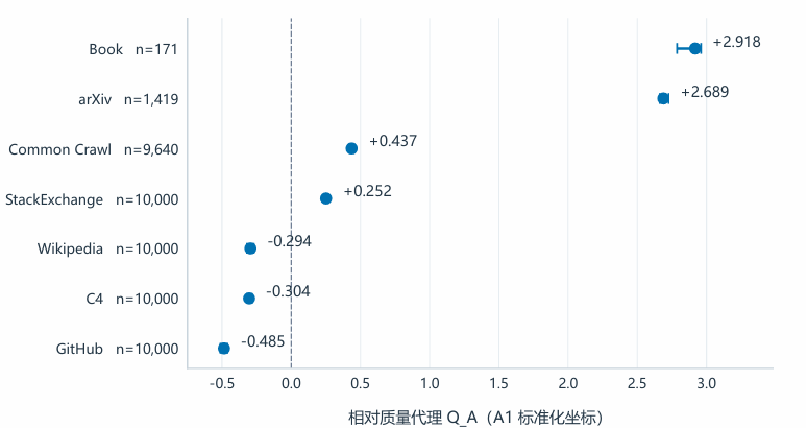
\includegraphics[width=0.94\linewidth]{figures/Q1/01_quality.pdf}
\caption{A1 七个来源域的相对质量评分中位数及抽样区间。}
 \label{fig:q1-quality}
\end{figure}

七个来源域的评分中位数见表\ref{tab:q1-quality}。Book 和 arXiv 分别为 2.9183 和 2.6887，明显高于其他来源域。A2、A3 全量评分中，arXiv 与 GitHub 的中位数分别为 2.7253 和 $-0.5055$；剔除与 A1 重叠的记录后分别为 2.7279 和 $-0.5063$，与抽样集结果相近。直接对 22 项指标等权时，Book、arXiv 仍居前，GitHub 仍居后，但 Wikipedia 与 C4 的相邻次序互换。留一来源域分析中还有 5 项指标的方向发生变化。另按来源域将 A1 划为 70\% 的方向拟合样本和 30\% 的检查样本，在拟合部分重复重抽 100 次，考察 14 项标量指标方向改变时的评分表现。图\ref{fig:q1-quality}中的区间反映文本重抽样，而这些比较反映评分规则选择的影响。由此可见，主要质量差异较清楚，相近来源域的排序仍会受赋权和指标方向影响。

\begin{table}[htbp]
 \centering\small
 \caption{A1 七个来源域的质量评分中位数}
 \label{tab:q1-quality}
 \begin{tabular}{lr@{\qquad}lr}
 \toprule
 来源域 & 质量评分 & 来源域 & 质量评分\\
 \midrule
 Book & 2.9183 & arXiv & 2.6887\\
 CommonCrawl & 0.4367 & StackExchange & 0.2517\\
 Wikipedia & $-0.2944$ & C4 & $-0.3040$\\
 GitHub & $-0.4854$ & & \\
 \bottomrule
 \end{tabular}
\end{table}

\subsubsection{指标分歧与复核规则}

综合评分可能掩盖同一文本上不同指标的分歧。对方向统一后的 22 项指标，计算全部 $\binom{22}{2}=231$ 个指标对的 Spearman 相关，并采用 Benjamini--Hochberg 方法\cite{fdr2019}将错误发现率控制在 0.05。A1 样本中有 66 对指标显著负相关，其中 55 对在去重后的 A2、A3 扩展数据中仍表现出相同的分歧方向，记为冲突指标对集合 $\mathcal E_c$。为衡量一条文本上这些指标给出的评价差异，定义分歧度
\begin{equation}
 D_i=\frac{\sum_{(u,v)\in\mathcal E_{c,i}}\lvert\rho_{uv}\rvert
 \lvert d_uz_{iu}-d_vz_{iv}\rvert}
 {\sum_{(u,v)\in\mathcal E_{c,i}}\lvert\rho_{uv}\rvert}.
 \label{eq:q1-disagreement}
\end{equation}
其中 $\mathcal E_{c,i}$ 为文本 $i$ 中两项指标均有值的冲突指标对，$\rho_{uv}$ 为相应的秩相关系数。$D_i$ 越大，表示该文本在相互冲突的指标上所得评价差异越大。当文本缺少可用的冲突指标对时，也将其列入复核。以 A1 的评分中位数 0.0273 划分筛选优先级，以分歧度的第 75 百分位 2.0423 作为复核阈值，得到优先保留、优先保留并复核、低优先级、低优先级并复核四类，分别包含 20,384、5,231、18,038 和 7,577 条文本。高分歧文本保留原有质量评分，同时增加复核标记。对原文的检查显示，公式宏、代码片段及较长的结构化文本容易使指标关注不同特征，这解释了部分文本同时获得较高质量评分与较大分歧度的现象。

图\ref{fig:q1-conflict}将评分高低与是否需要复核交叉展示。对 27 条原文案例的逐条查看有助于解释指标分歧产生的文本特征；这些案例没有人工质量标签，因而这里评价的是规则的可解释性，而非分类准确率。分歧阈值用于安排复核，未将高分歧直接等同于低质量。

\begin{figure}[htbp]
 \centering
 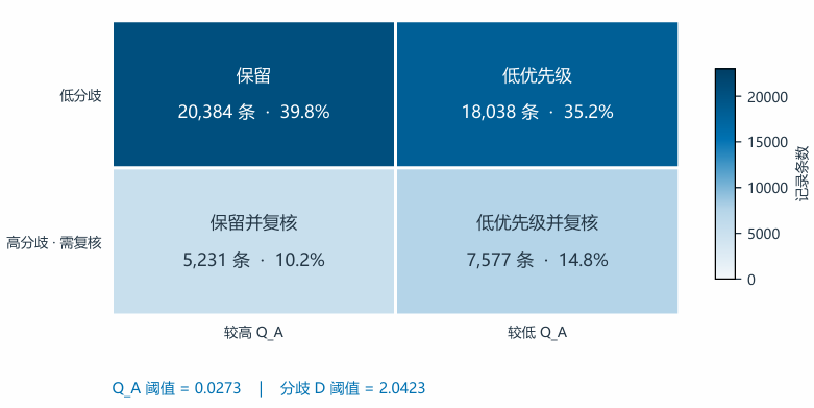
\includegraphics[width=0.88\linewidth]{figures/Q1/02_conflict.pdf}
 \caption{综合质量评分与指标分歧度共同形成的文本筛选结果}
 \label{fig:q1-conflict}
\end{figure}

\subsection{领域配比建模与验证}

\subsubsection{二阶交互模型}

记 The Pile\cite{pile2022} 的 17 个训练子领域份额为 $\boldsymbol p=(p_1,\ldots,p_{17})^\mathsf T$。对 A4 中因小数舍入而存在微小总和偏差的配比归一化后，满足 $p_j\geqslant0$ 且 $\sum_jp_j=1$；第 $k$ 个验证域的 Loss 记为 $L_k$，其中 $k=1,\ldots,13$。考虑到领域组合可能影响训练效果\cite{regmix2025,mixinglaws2025}，在 17 个份额主项之外，根据训练域配比的样本方差选取变化最大的 5 个领域，构造 10 个两两交互项。对每个验证域分别建立模型：
\begin{equation}
 \widehat L_k(\boldsymbol p)=a_k+\sum_{j=1}^{17}b_{kj}p_j
 +\sum_{(u,v)\in\mathcal E} \gamma_{k,uv}p_up_v,
 \qquad\lvert\mathcal E\rvert=10.
 \label{eq:q1-mixture}
\end{equation}
入选领域为 FreeLaw、arXiv、PubMed Central、GitHub 和 Pile-CC。模型对非截距系数施加 $L_2$ 正则，并通过五折交叉验证逐验证域选择正则强度；以仅含 17 个主项的岭回归模型和训练均值预测作为对照\cite{islr2021}。拟合结果中，arXiv 与 GitHub、arXiv 与 Pile-CC 的交互项在 13 个验证域上均为负，表明这些领域组合与较低的预测 Loss 相联系。十个领域组合在 13 个验证域上共有 130 个交互系数，其中 110 个在五次分折拟合中始终保持全样本的符号，反映主要组合关系具有一定稳定性。由于各域份额之和恒为 1，增加一个领域的训练比例必然伴随其他领域比例下降，因而对模型系数的分析需结合具体的配比转移方向。

图\ref{fig:q1-pair-contributions}在参考配比处比较十个交互项对不同验证域预测的贡献。同一领域组合的贡献幅度随验证域改变，说明只看某一训练域的单独份额不足以解释全部 Loss 变化。图中的乘积项贡献是给定配比处的模型分解；真正调整配比时，仍须同时计算被减配领域的变化。

\begin{figure}[htbp]
 \centering
 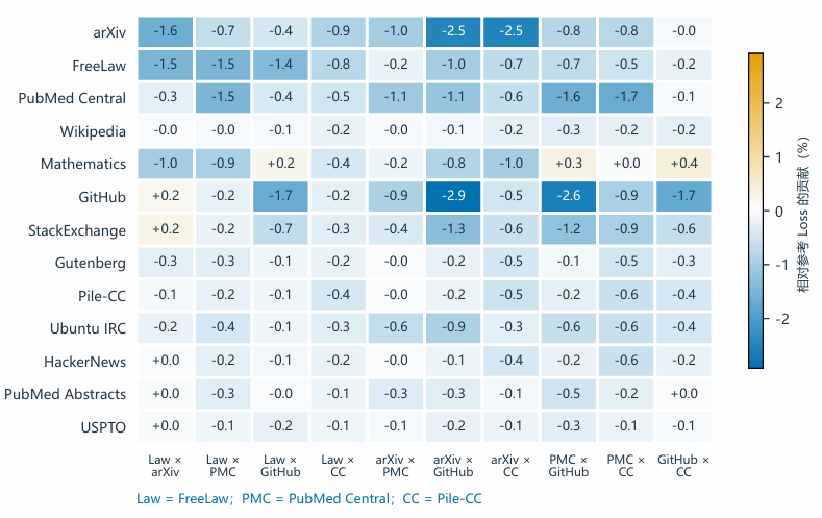
\includegraphics[width=0.94\linewidth]{figures/Q1/08_pair_contributions.pdf}
 \caption{参考配比处十个领域交互项对各验证域预测 Loss 的贡献}
 \label{fig:q1-pair-contributions}
\end{figure}

以 A4 的平均配方 $\boldsymbol p_{\mathrm{ref}}$ 为参照，定义第 $k$ 个验证域的相对 Loss 变化：
\begin{equation}
 r_k(\boldsymbol p)=
 \frac{\widehat L_k(\boldsymbol p)-\widehat L_k(\boldsymbol p_{\mathrm{ref}})}
 {\widehat L_k(\boldsymbol p_{\mathrm{ref}})},
 \label{eq:q1-relative}
\end{equation}
式\eqref{eq:q1-relative}使不同验证域的 Loss 变化具有可比性；$r_k(\boldsymbol p)<0$ 表示相对参考配方的预测 Loss 降低。组合项 $\gamma_{k,uv}p_up_v$ 则刻画所选领域配比之间的非加性关系，其作用随验证域和当前配方而变化。

\subsubsection{模型检验与外推分析}

采用五折嵌套交叉验证比较模型\cite{hpo2023}，外层留出样本用于计算误差，内层重新选择交互领域和正则强度。交互模型在 13 个验证域上的均方根误差（RMSE）均低于岭回归，中位数由 0.4921 降至 0.4499，表明交互项有助于描述配比与 Loss 的关系。在 A6--A11 检验组中，1M、60M 和 1B 分别有 11、13、13 个验证域的 RMSE 低于同组岭回归，见图\ref{fig:q1-validation}。1M 与 60M 组使用相同的 256 个配方，比较的是规模变化下同一组成集合的表现；1B 组有 47/64 个配方位于 A4 配方凸包之外，也考察了对新配比的预测。A6--A11 的比较参与了模型形式的选择，故这里将其用于说明选择交互模型的依据；嵌套交叉验证则用于评价逐折重新选择特征后的预测误差。

\begin{figure}[htbp]
 \centering
 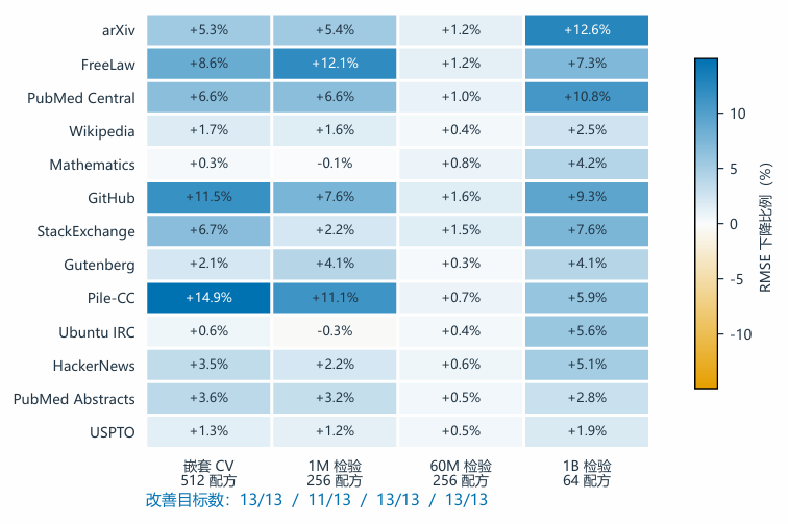
\includegraphics[width=0.94\linewidth]{figures/Q1/03_validation.pdf}
 \caption{交互模型相对岭回归在各验证域上的 RMSE 变化}
 \label{fig:q1-validation}
\end{figure}

进一步比较模型预测与各实验组实测 Loss 对配方的排序。1M、60M、1B 三组在 13 个验证域上的 Spearman 相关中位数分别为 0.851、0.847、0.791，说明模型在给定检验组中较好地保持了配方的相对顺序。对于附件估算的 10B、70B Loss，相关中位数降至 0.492 和 0.394，略低于同组线性岭回归的 0.514 和 0.415，如图\ref{fig:q1-rank}所示。在两张外推表共同包含的 63 个配方中，按 1M 模型等权目标选出的同一配方，在两组估算 Loss 中均排第 61 位。这一反向比较表明，交互模型在较大规模估算表上的排序优势未能延续。后两组 Loss 来自估算，主要用于考察外推趋势；跨规模应用时仍需结合新的实验数据校准。

\begin{figure}[htbp]
 \centering
 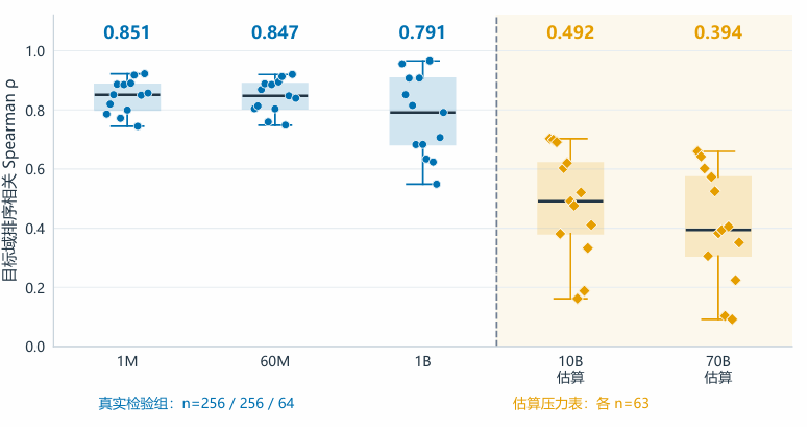
\includegraphics[width=0.91\linewidth]{figures/Q1/04_rank_stress.pdf}
 \caption{配比模型在检验组及外推表上的逐验证域排序相关}
 \label{fig:q1-rank}
\end{figure}

\subsection{质量约束下的配比方案}

\subsubsection{目标函数与约束}

为在已有配比实验覆盖的范围内调整训练组成，取 A4 中 512 个配方的凸包为搜索区域\cite{wright2022}：
\begin{equation}
 \mathcal P_A=\left\{\boldsymbol p=\sum_{i=1}^{512}\omega_i\boldsymbol p^{(i)}:
 \omega_i\geqslant0,\ \sum_i\omega_i=1\right\}.
 \label{eq:q1-hull}
\end{equation}

考虑两种目标偏好。等权平均目标关注 13 个验证域的总体改善，最大相对 Loss 目标关注最不利验证域：
\begin{equation}
 F_{\mathrm{avg}}(\boldsymbol p)=\frac1{13}\sum_{k=1}^{13}r_k(\boldsymbol p),
 \qquad F_{\mathrm{max}}(\boldsymbol p)=\max_k r_k(\boldsymbol p).
 \label{eq:q1-objectives}
\end{equation}
质量信号的七个来源域与 17 个训练域之间没有完整的一一对应关系。参照 A16，分别考察仅采用直接映射、同时采用直接映射与近似直接映射两种质量约束。记 $J$ 为相应可映射训练域的集合，$q_j$ 为对应来源域的质量评分，$M_J(\boldsymbol p)=\sum_{j\in J}p_j$ 为这些领域的总份额。参考配方在该部分的平均质量为
\begin{equation}
 \bar q_{J,0}=
 \frac{\sum_{j\in J}p_{\mathrm{ref},j}q_j}
 {M_J(\boldsymbol p_{\mathrm{ref}})}.
 \label{eq:q1-reference-quality}
\end{equation}
约束写为
\begin{equation}
 M_J(\boldsymbol p)\geqslant M_J(\boldsymbol p_{\mathrm{ref}}),\qquad
 \sum_{j\in J}p_j(q_j-\bar q_{J,0})\geqslant0.
 \label{eq:q1-quality-constraint}
\end{equation}
式\eqref{eq:q1-quality-constraint}要求可映射领域的总份额和平均质量均不低于参考配方。对仅有推断映射的其余 11 个领域，不直接赋予来源域质量评分。由于式\eqref{eq:q1-mixture}含双线性项，本文采用 McCormick 松弛与空间分支定界求解\cite{global2025}：节点上的线性规划给出目标下界，相应的凸组合生成可行配方和目标上界。以 0.001 的目标上下界差为停止阈值。另在 512 个原始配方中逐一比较，得到只从现有配方中选择时的方案。

\subsubsection{求解结果与配方分析}

四种情景的结果见表\ref{tab:q1-policy}，连续配方求解的目标上下界差均小于 0.001。以等权平均 Loss 为目标时，加入质量约束后，相对参考配方的预测改善幅度由约 11.5\% 变为约 10.3\% 或 9.7\%，体现了降低 Loss 与维持数据质量之间的取舍。仅采用直接映射约束的连续配方中，arXiv、DM Mathematics、GitHub、Pile-CC、Ubuntu IRC 的训练份额约为 16.9\%、21.2\%、15.4\%、13.7\%、11.8\%；若只能选用 A4 中的原始配方，对应编号为 301。图\ref{fig:q1-recipes}展示了完整的 17 域份额。相比参考配方的 11.3\%，arXiv 在直接映射约束下升至 16.9\%，同时加入近似直接映射后升至 17.9\%。以最大相对 Loss 为优化目标时，所得配方在更多领域间分配份额，反映了对各验证域表现的均衡考虑。

\begin{table}[htbp]
 \centering\small
 \caption{不同目标与质量约束下的连续及原始配方结果；目标值为相对参考配方的变化}
 \label{tab:q1-policy}
 \resizebox{\linewidth}{!}{%
 \begin{tabular}{lrrrr}
 \toprule
 目标与质量约束 & 连续配方目标值 & 上下界差 & 原始配方编号 & 原始配方目标值\\
 \midrule
 等权平均，不设质量约束 & $-0.115112$ & 0.000962 & 136 & $-0.115065$\\
 等权平均，仅采用直接映射 & $-0.102992$ & 0.000441 & 301 & $-0.051923$\\
 等权平均，加入近似直接映射 & $-0.097010$ & 0.000750 & 172 & $-0.067371$\\
 最小化最大变化，不设质量约束 & $-0.019784$ & 0.000996 & 477 & $+0.039927$\\
 \bottomrule
 \end{tabular}
 }
\end{table}

\begin{figure}[htbp]
 \centering
 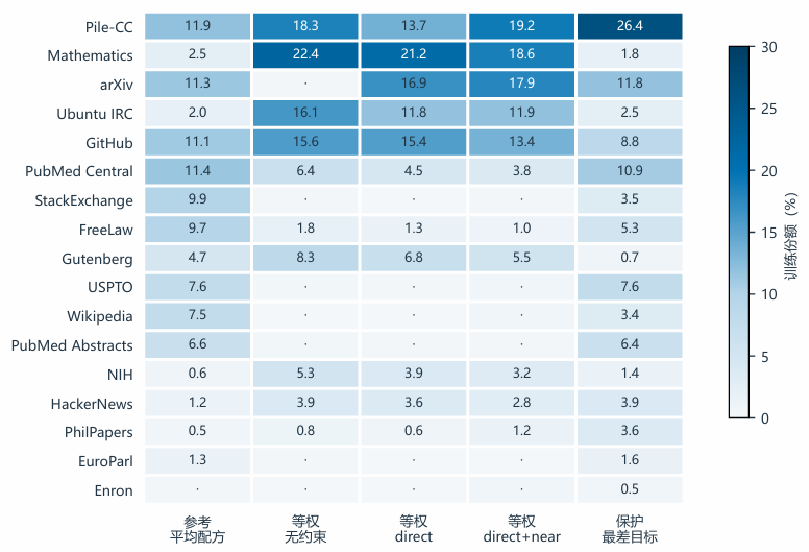
\includegraphics[width=0.94\linewidth]{figures/Q1/05_recipes.pdf}
 \caption{参考配方与不同目标下连续配方的 17 域训练份额}
 \label{fig:q1-recipes}
\end{figure}

表\ref{tab:q1-policy}中的原始配方编号对应的是在 512 个给定配方中选出的方案，而连续目标值来自整个凸包；两列结果应分别比较。特别是保护最不利验证域时，连续配方的最大相对 Loss 约为 $-0.0198$，原始配方中最优方案仍为 $+0.0399$，说明在已有配方之间作凸组合有助于改善这一均衡目标。

图\ref{fig:q1-policy-diagnostic}给出四种方案对各验证域 Loss 的预测变化。等权且不设质量约束的连续方案在 Mathematics 验证域得到 $-0.0901$ 的预测 Loss。交叉熵 Loss 应为非负值，说明二阶模型在这一配比区域发生了预测失真；这一数值不作为实际 Loss 收益。其余三个连续方案的逐域预测 Loss 均为正值。后续优化可加入非负约束或收紧搜索区域。

\begin{figure}[htbp]
 \centering
 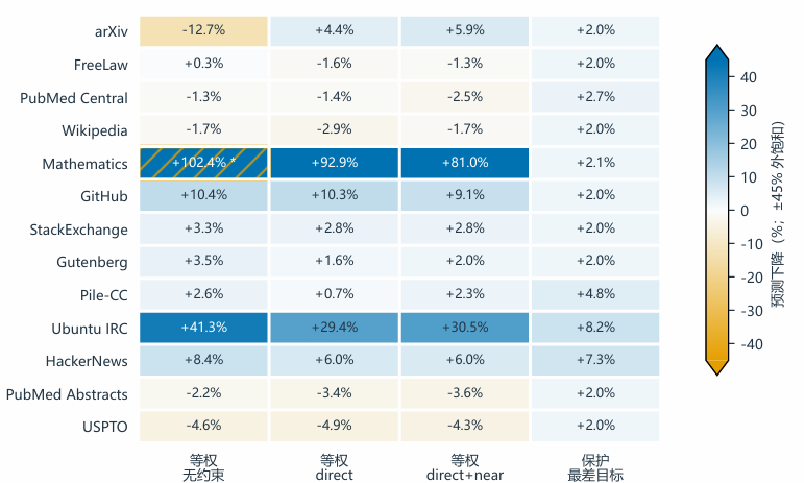
\includegraphics[width=0.94\linewidth]{figures/Q1/06_policy_results.pdf}
 \caption{四种配比方案的逐验证域预测变化；斜线格标出负预测 Loss}
 \label{fig:q1-policy-diagnostic}
\end{figure}

为考察配方选择对样本扰动的敏感性，进行 30 次重复子采样，每次抽取 80\% 的 A4、A5 配对样本，重新选择交互领域和正则强度、拟合模型，再从 512 个原始配方中选取方案。四种情景中原配方再次被选中的次数依次为 29、10、13、7 次，见图\ref{fig:q1-stability}。无质量约束的等权方案选择较稳定；加入质量约束或改用最大相对 Loss 目标后，具体配方对样本扰动更敏感。因此，领域配比的选择应同时说明质量条件和目标偏好。

\begin{figure}[htbp]
 \centering
 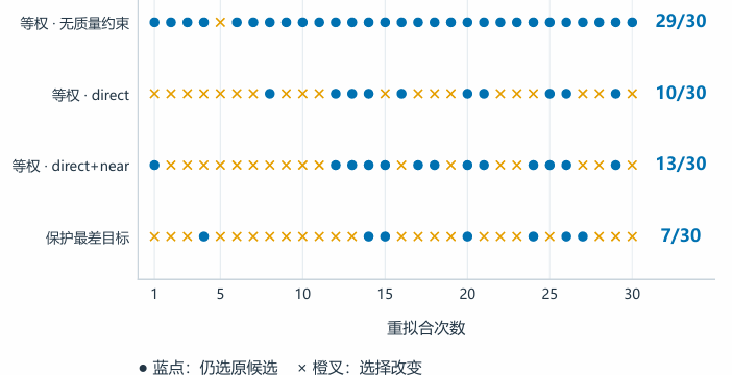
\includegraphics[width=0.85\linewidth]{figures/Q1/07_stability.pdf}
 \caption{30 次重复子采样中原始配方再次被选中的频率}
 \label{fig:q1-stability}
\end{figure}

\subsection{本问结果与后续衔接}

第一问得到的质量评分与配比关系来自不同数据：$Q_A$ 描述来源域质量信号的相对水平，$r_k(\boldsymbol p)$ 描述 A4、A5 中第 $k$ 个验证域相对参考配方的 Loss 变化。表\ref{tab:q1-output}汇总了进入下一问的主要量。两套数据缺少相同训练实验下的成对观测，因此下一问需要明确建立质量尺度与 Loss 口径之间的连接假设。

\begin{table}[htbp]
 \centering\small
 \caption{第一问的主要输出及其在广义标度律中的作用}
 \label{tab:q1-output}
 \begin{tabular}{p{0.20\linewidth}p{0.35\linewidth}p{0.35\linewidth}}
 \toprule
 输出 & 本问含义 & 后续使用方式\\
 \midrule
 $Q_A$ 及域级中位数 & A1--A3 上统一方向后的相对质量评分 & 经 A16 的直接及近似直接映射，构造训练配比的质量输入\\
 $r_k(\boldsymbol p)$ & 13 个验证域相对参考配比的 Loss 变化 & 按目标域偏好加权后描述配比对 Loss 的相对影响\\
 $\mathcal P_A$ 与映射范围 & 512 个配方的凸包及有质量评分的训练域 & 约束配比取值，并保留未映射领域的质量缺失\\
 \bottomrule
 \end{tabular}
\end{table}

\subsection{本问小结}

本问利用 A1--A3 的全部质量信号建立了样本评分与域级质量评分，并以指标分歧度识别需要复核的文本；扩展样本与抽样集给出了相近的 arXiv、GitHub 域级结果。基于 512 组训练配比建立的二阶交互模型，在 13 个验证域上的交叉验证误差均低于线性岭回归，并在 1M、60M、1B 检验组中较好地保持了配方排序。结合来源域与训练域的参考映射，可以得到不同质量要求及目标偏好下的领域配比。上述结果刻画了数据质量、领域组成与验证 Loss 之间的定量关系，为训练数据筛选和配比调整提供了依据。

\setcounter{section}{4}
\section{问题二：跨维度数据融合与广义标度律}
\label{sec:q2}
\setcounter{equation}{0}
\setcounter{figure}{0}
\setcounter{table}{0}

\subsection{问题分析}

经典标度律以模型参数量 $N$ 和训练数据量 $D$ 描述验证集交叉熵损失（Loss）\cite{kaplan2020scaling,hoffmann2022training}，但未反映数据质量和训练领域组成。本问需要将第一问得到的质量评分与领域配比关系接入规模模型，进而分析各因素的边际效用，以及提高数据质量与扩大模型规模的替代条件。由于附件 A 与附件 B 来自不同实验，两组质量指标和 Loss 的数值口径并不相同，本文分别估计附件 B 中的规模关系和质量关系，再以第一问的相对配比效应建立跨来源的统一表达式。

全文令 $N$ 以十亿参数、$D$ 以十亿 Token 计。B1 的 1176 条 Pythia\cite{pythia2023} 训练记录用于估计 $N$--$D$ 标度律；B7 的 450 条半合成记录用于估计质量项。B6 的实验点包含于 B7，B8 的质量变化趋势与 B7 不一致，因此二者不重复用于本次质量拟合。B2、B3 检查不同轨迹上的变化趋势，B4、B5 比较跨模型族及文献数据中的下降方向；B9、B10 用于讨论大规模外推，B11、B12 提供模型族和检查点的辅助信息。第一问的质量评分和 17 维训练配比通过其已有结果引入，本问不重新处理附件 A 的原始数据。

\subsection{经典标度律的建立}

\subsubsection{模型形式与参数估计}

以 B1 的模型参数量、累计训练 Token 数和验证 Loss 为观测量，建立经典双幂律\cite{hoffmann2022training}
\begin{equation}
 L_0(N,D)=E+A N^{-\alpha}+B D^{-\beta},
 \qquad E,A,B,\alpha,\beta>0.
 \label{eq:q2-classic}
\end{equation}
其中 $E$ 表示规模继续增大时的渐近项，两个幂律项分别描述参数量与训练量带来的 Loss 变化。为避免某一参数规模的密集检查点主导拟合，对 B1 的八个模型规模组赋予相同总权重，以对数 Loss 残差的 Huber 损失估计参数，并在正参数约束下采用多起点搜索。所得结果为
\begin{equation}
 L_0(N,D)=1.689838+0.353969N^{-0.339985}
              +1.240275D^{-0.279892}.
 \label{eq:q2-classic-fit}
\end{equation}
两个指数均为正，因此在模型考察范围内，增加 $N$ 或 $D$ 都会降低预测 Loss。

B1 全样本 RMSE 为 $1.466\times10^{-4}$；按模型规模留一组检验的平均 RMSE 为 $1.461\times10^{-4}$，各规模组最后 30\% 训练阶段留出的 RMSE 为 $1.160\times10^{-4}$。作为形式对照，直接对 $\ln N$ 和 $\ln D$ 作线性回归的全样本 RMSE 为 0.1030，明显高于双幂律。图\ref{fig:q2-baseline}展示了拟合值与记录值的关系。三种检验的误差量级相近，说明式\eqref{eq:q2-classic-fit}较稳定地重现了 B1 的规模轨迹。图\ref{fig:q2-scale-surface}进一步给出其在主要取值范围内的 Loss 曲面：当其中一项资源已经较大时，继续增加该项资源所带来的下降逐渐变缓。

\begin{figure}[htbp]
 \centering
 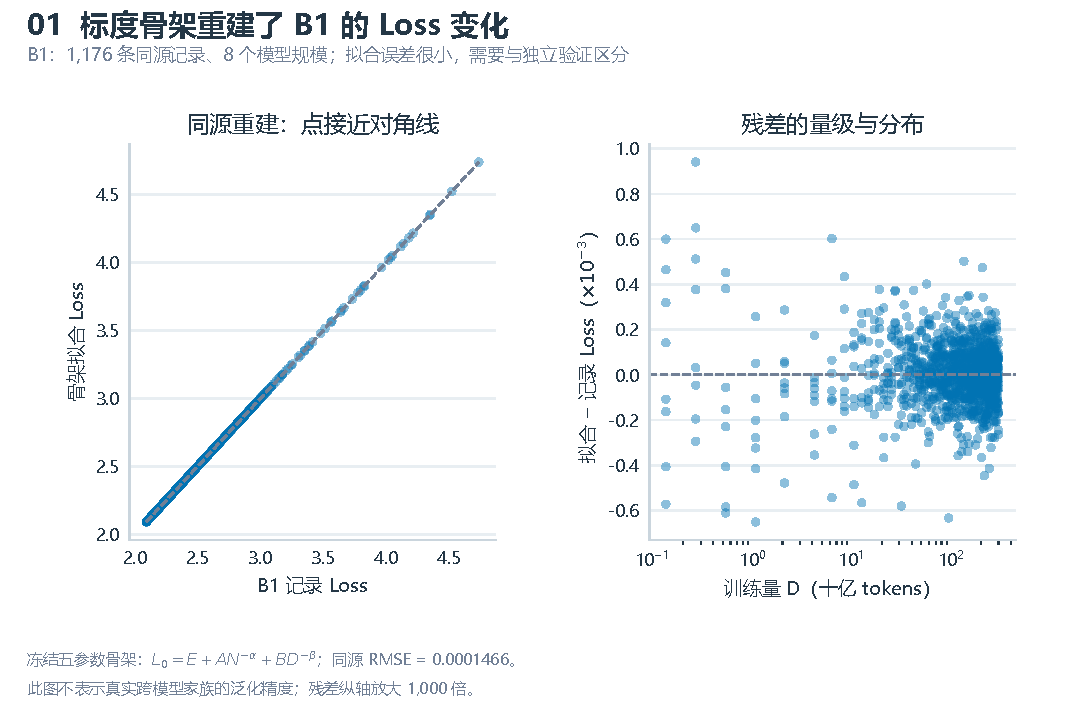
\includegraphics[width=0.90\linewidth]{figures/Q2/01_baseline.pdf}
 \caption{B1 训练记录中经典标度律的拟合值与残差}
 \label{fig:q2-baseline}
\end{figure}

\begin{figure}[htbp]
 \centering
 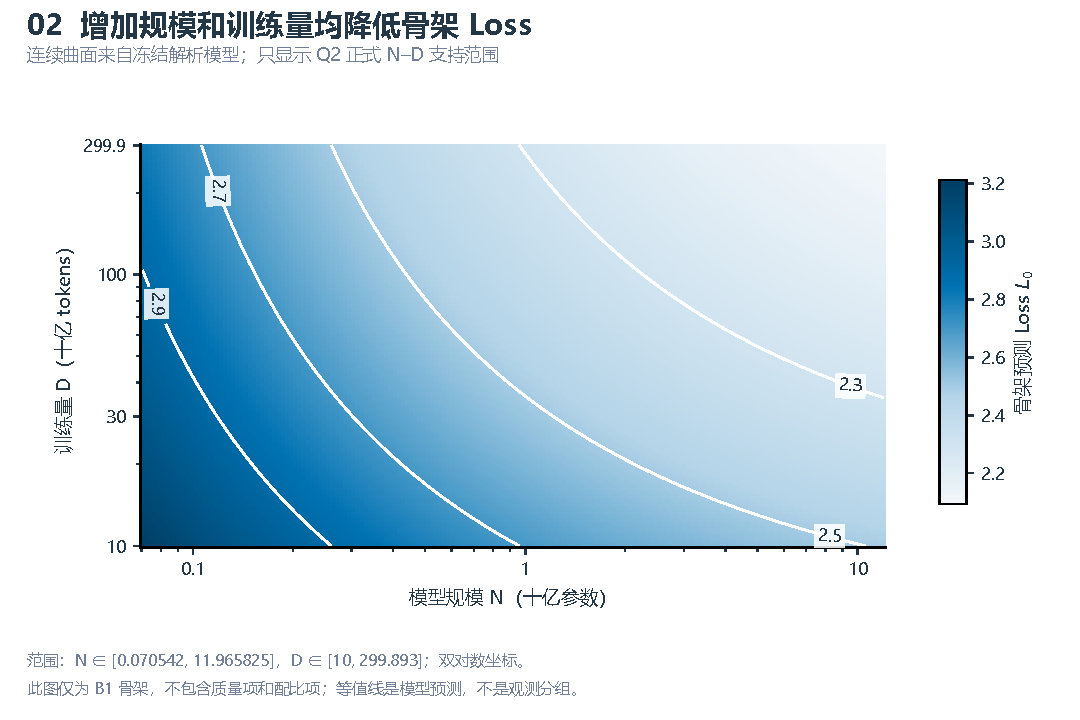
\includegraphics[width=0.88\linewidth]{figures/Q2/02_scale_surface.pdf}
 \caption{经典标度律在模型参数量与训练量范围内的预测 Loss 曲面}
 \label{fig:q2-scale-surface}
\end{figure}

\subsubsection{规模关系的跨数据检验}

将式\eqref{eq:q2-classic-fit}用于 B3 的八条 Pythia 插值轨迹和 B2 的七条 Cerebras 半合成轨迹，按各轨迹自身尺度计算的平均归一化 RMSE 分别为 0.001892 和 0.004370；相应的配对排序一致率为 0.9991 和 0.9855。B4 与 B5 中，在共同规模范围内可比较的同族规模配对分别有 12 对和 7 对，Loss 下降方向全部一致。这些结果表明模型捕捉到了随规模和训练量增加而降低 Loss 的主要趋势。由于各来源的验证语料和 Loss 口径未统一，跨来源检验主要用于比较轨迹形状与下降方向。

\subsection{数据质量与领域配比的融合}

\subsubsection{质量项的估计}

B7 提供了具有质量评分 $Q_B$ 的半合成实验。在相同 $(N,D)$ 组合下检查质量与 Loss 的关系时，单一固定质量斜率难以描述全部规模水平，组级误差约为 0.1078。为使质量效应随规模改变，并保持 B1 的规模参数不变，本文在式\eqref{eq:q2-classic-fit}上添加质量项：
\begin{align}
 L_B(N,D,Q_B)&=L_0(N,D)+(1-Q_B)G(N,D),\label{eq:q2-quality}\\
 G(N,D)&=G_0+G_N\ln N+G_D\ln(D/100).\label{eq:q2-gain}
\end{align}
当 $Q_B=1$ 时，质量项为零，模型回到经典标度律。$G(N,D)$ 则允许质量改进的效果随规模和训练量变化。固定 B1 的五个参数，仅用 B7 估计得到
\begin{equation}
 G(N,D)=0.371703-0.061115\ln N-0.014961\ln(D/100).
 \label{eq:q2-gain-fit}
\end{equation}
在 B7 考察的矩形范围内，$G(N,D)$ 的最小值为 0.193184，故提高 $Q_B$ 对应预测 Loss 下降。B7 的 450 条数据并非独立的大模型训练实测，式\eqref{eq:q2-gain-fit}描述的是该半合成数据所体现的质量变化规律。

为检验质量项，分别留出一个 $N$、$D$ 或 $Q_B$ 水平，重新选择正则强度并估计参数。24 个外层折的平均 RMSE 依次为 0.048738、0.048751、0.048639，三种留出方式得到相近结果，见图\ref{fig:q2-quality-validation}。表\ref{tab:q2-quality-models}将三参数质量扩展与在 B7 上联合估计全部八个参数的方案并列展示。后者训练误差略小，但留出水平上的误差较大；固定 B1 主干也使两组数据各自承担的估计任务更清楚。两种方案的留出选参流程不同，表中比较用于判断模型复杂度与误差的取舍。

\begin{table}[htbp]
 \centering\small
 \caption{B7 半合成数据中两种质量扩展方式的预测误差（RMSE）}
 \label{tab:q2-quality-models}
 \begin{tabular}{lrrrr}
 \toprule
 模型 & 训练样本 & 留 $N$ 水平 & 留 $D$ 水平 & 留 $Q_B$ 水平\\
 \midrule
 固定 B1，仅估计三项质量参数 & 0.048540 & 0.048738 & 0.048751 & 0.048639\\
 B7 联合估计八项参数 & 0.048410 & 0.049764 & 0.049008 & 0.049352\\
 \bottomrule
 \end{tabular}
\end{table}

\begin{figure}[htbp]
 \centering
 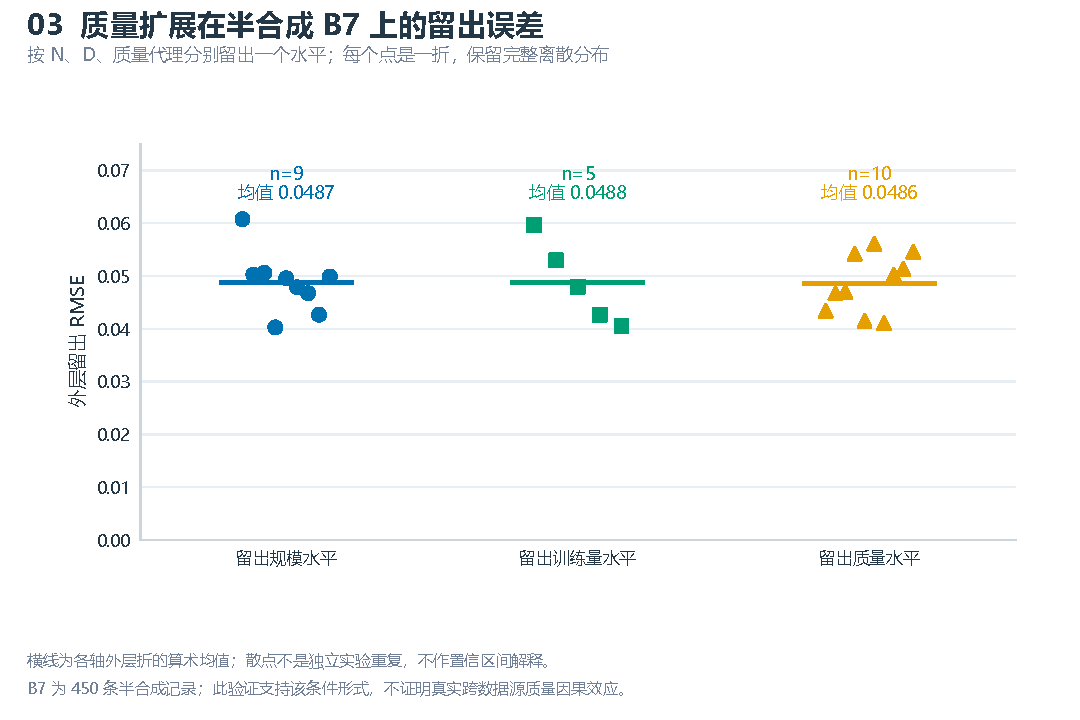
\includegraphics[width=0.88\linewidth]{figures/Q2/03_quality_validation.pdf}
 \caption{B7 半合成数据中按规模、训练量和质量水平留出的预测误差}
 \label{fig:q2-quality-validation}
\end{figure}

\subsubsection{质量评分与配比效应的连接}

第一问给出的来源域质量评分记为 $q_{A,j}$，17 个训练域的配比为 $\boldsymbol p=(p_1,\ldots,p_{17})^\mathsf T$。根据 A16 的参考映射，取具有直接映射或近似直接映射的六个训练域组成集合 $\mathcal M$，并按其在配比中的份额计算平均质量：
\begin{equation}
 Q_A(\boldsymbol p)=
 \frac{\sum_{j\in\mathcal M}p_jq_{A,j}}
      {\sum_{j\in\mathcal M}p_j},
 \qquad \sum_{j\in\mathcal M}p_j>0.
 \label{eq:q2-qa}
\end{equation}
没有对应质量评分的训练域不补造数值。由于 $Q_A$ 与 B7 的 $Q_B$ 采用不同尺度，以六个可映射领域评分的最小值 $q_{\min}$ 和最大值 $q_{\max}$ 定义保序映射
\begin{equation}
 q(\boldsymbol p)=\Pi_{[0.1,1]}\!\left[
 0.1+0.9\frac{Q_A(\boldsymbol p)-q_{\min}}
 {q_{\max}-q_{\min}}\right],
 \label{eq:q2-quality-map}
\end{equation}
其中 $\Pi_{[0.1,1]}$ 表示将数值限制在 B7 的质量范围内。该映射保留第一问评分的相对次序；参考配比对应 $Q_A=0.783104$、$q=0.435406$，其斜率将在后文作敏感性分析。

记第一问对第 $k$ 个验证域的配比预测为 $\widehat L_{A,k}(\boldsymbol p)$，以 A4 的平均配比 $\boldsymbol p_{\mathrm{ref}}$ 为参照，构造相对变化
\begin{equation}
 r_k(\boldsymbol p)=
 \frac{\widehat L_{A,k}(\boldsymbol p)
       -\widehat L_{A,k}(\boldsymbol p_{\mathrm{ref}})}
      {\widehat L_{A,k}(\boldsymbol p_{\mathrm{ref}})},
 \qquad
 r_{\boldsymbol w}(\boldsymbol p)=\sum_{k=1}^{13}w_kr_k(\boldsymbol p),
 \quad \sum_{k=1}^{13}w_k=1,\ w_k\geqslant0.
 \label{eq:q2-mixture-effect}
\end{equation}
权重 $w_k$ 表示对 13 个验证域的重视程度，主结果取等权。$r_{\boldsymbol w}(\boldsymbol p_{\mathrm{ref}})=0$，因此参考配比为跨来源连接提供了明确的零变化点。

\subsubsection{广义标度律}

将规模、质量和配比三部分结合，得到本问的广义标度律：
\begin{equation}
 \boxed{\widehat L(N,D,q,\boldsymbol p;\boldsymbol w)
 =\left[L_0(N,D)+(1-q)G(N,D)\right]
       \exp\!\bigl\{r_{\boldsymbol w}(\boldsymbol p)\bigr\}.}
 \label{eq:q2-general}
\end{equation}
在依据第一问质量评分的主情景中，$q=q(\boldsymbol p)$，质量随配比共同变化；讨论额外改善数据质量时，则固定配比，把 $q$ 作为单独变化的质量坐标。指数形式保证配比修正始终为正，并使参考配比的修正系数等于 1。$q=1$ 时质量项消失；若同时取参考配比，式\eqref{eq:q2-general}退化为式\eqref{eq:q2-classic}。质量评分与配比效应来自不同实验，式\eqref{eq:q2-quality-map}的尺度映射及指数形式是跨来源连接假设，其数值影响由后文的斜率敏感性分析检验。

模型在共同数据范围内考察 $N\in[0.070542,11.965825]$、$D\in[10,299.893]$、$q\in[0.1,1]$，配比取 A4 原始配方或其凸包内的可行点。B7 中有 240 条记录的 $N$ 或 $D$ 位于 B1 的范围之外；它们参与质量项估计，但最终预测采用两组数据的共同范围。以 $N=1$、$D=100$、13 个验证域等权为例，在满足直接及近似直接映射质量条件的 108 个原始配方中，配方 172 的 $Q_A=1.675449$、$q=0.671361$，预测 Loss 为 2.344348。该数值展示了式\eqref{eq:q2-general}如何把四类因素合并到同一计算框架中。

\subsection{边际效用与弹性}

为比较四类因素的局部作用，设 $H=L_0+(1-q)G$、$F=\exp\{r_{\boldsymbol w}(\boldsymbol p)\}$。固定配比和质量坐标时，式\eqref{eq:q2-general}对规模、训练量与质量的偏导数为
\begin{align}
 \frac{\partial\widehat L}{\partial N}
 &=F\left[-\alpha AN^{-\alpha-1}
             +(1-q)\frac{G_N}{N}\right],\label{eq:q2-marginal-n}\\
 \frac{\partial\widehat L}{\partial D}
 &=F\left[-\beta BD^{-\beta-1}
             +(1-q)\frac{G_D}{D}\right],\label{eq:q2-marginal-d}\\
 \frac{\partial\widehat L}{\partial q}&=-FG(N,D).\label{eq:q2-marginal-q}
\end{align}
若质量由配比决定，则沿第 $j$ 个训练域的份额方向还有
\begin{equation}
 \frac{\partial\widehat L}{\partial p_j}
 =F\left[H\frac{\partial r_{\boldsymbol w}}{\partial p_j}
       -G\frac{\partial q}{\partial p_j}\right].
 \label{eq:q2-marginal-p}
\end{equation}
式\eqref{eq:q2-marginal-p}将配比变化对质量评分及验证域 Loss 的两条作用途径同时计入。由于配比总和恒为 1，实际分析采用一个领域增加、另一个领域减少的可行方向。

定义 Loss 下降弹性 $\varepsilon_x=-x(\partial\widehat L/\partial x)/\widehat L$。它表示 $x$ 局部增加 1\% 时，Loss 约下降 $\varepsilon_x$\%。取上一节的配方 172、$D=100$、$q=0.671361$，结果见表\ref{tab:q2-elasticity}与图\ref{fig:q2-elasticity}。当 $N$ 从 0.1 增至 10 时，参数弹性由 0.0953 降至 0.0331，而质量弹性由 0.1157 降至 0.0683；同一配方下，参数量的相对边际收益随规模增加而减弱。

\begin{table}[htbp]
 \centering\small
 \caption{固定配方、$D=100$ 时各因素的局部 Loss 下降弹性}
 \label{tab:q2-elasticity}
 \begin{tabular}{rrrrr}
 \toprule
 $N$（十亿参数） & 预测 Loss & $\varepsilon_N$ & $\varepsilon_D$ & $\varepsilon_q$\\
 \midrule
 0.1 & 2.780596 & 0.095267 & 0.033814 & 0.115662\\
 1 & 2.344348 & 0.055998 & 0.040106 & 0.099511\\
 10 & 2.121466 & 0.033091 & 0.044320 & 0.068334\\
 \bottomrule
 \end{tabular}
\end{table}

\begin{figure}[htbp]
 \centering
 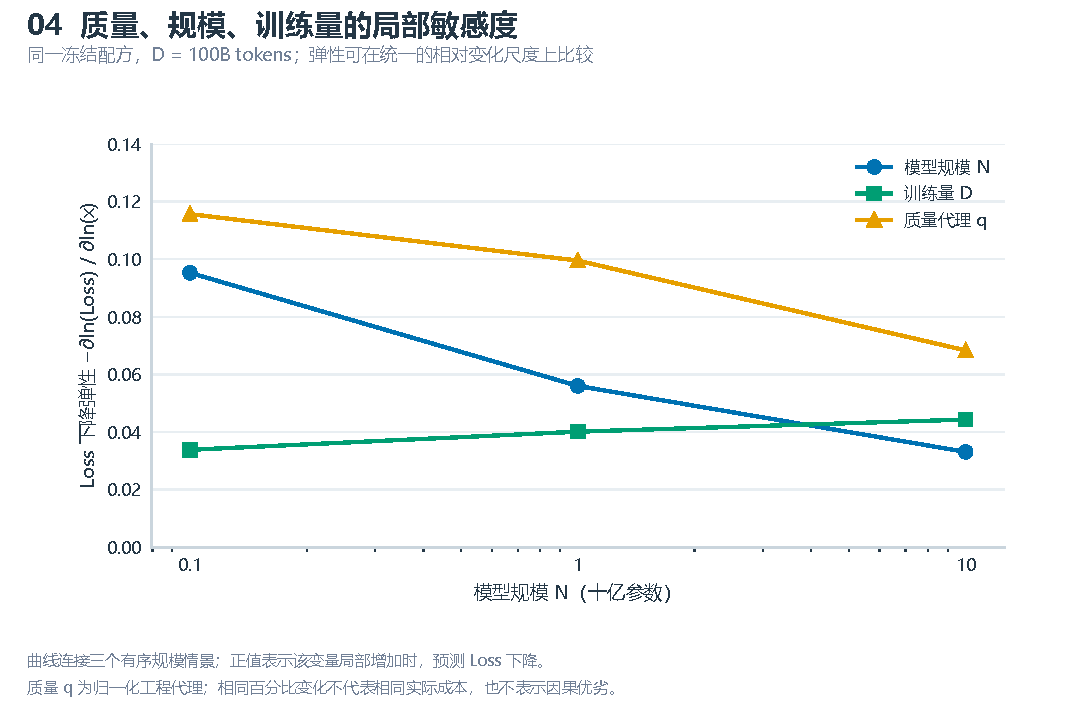
\includegraphics[width=0.86\linewidth]{figures/Q2/04_elasticities.pdf}
 \caption{固定训练量和配比时参数量、训练量与质量的局部弹性}
 \label{fig:q2-elasticity}
\end{figure}

弹性比较的是相同百分比变化，并未考虑资源成本。若提高参数量和质量的边际成本分别为 $C_N$、$C_q$，则同一位置每单位成本带来的 Loss 降低量分别为 $-\widehat L_N/C_N$ 与 $-\widehat L_q/C_q$。前者较大时增加参数量更合算，后者较大时改善质量更合算。这一判据为加入具体质量处理成本后的资源分配提供了直接依据。

\subsection{质量提升与模型规模的替代}

固定 $D$ 与配比，令质量坐标发生独立变化，并沿等 Loss 曲线对式\eqref{eq:q2-general}求微分，可得
\begin{equation}
 \frac{\mathrm dN}{\mathrm dq}
 =-\frac{\widehat L_q}{\widehat L_N}.
 \label{eq:q2-tradeoff}
\end{equation}
在所考察的范围内，$\widehat L_q$ 与 $\widehat L_N$ 均为负，因此 $\mathrm dN/\mathrm dq<0$：提高质量后，可以用较小的模型维持原有 Loss。对于有限增量 $\Delta q$，应分别求解“旧质量下扩模达到同样 Loss”和“提高质量后缩模维持原 Loss”两个方程：
\begin{equation}
 \begin{aligned}
 \widehat L(N_{\mathrm{eq}},D,q,\boldsymbol p)
   &=\widehat L(N,D,q+\Delta q,\boldsymbol p),\\
 \widehat L(N_{\mathrm{new}},D,q+\Delta q,\boldsymbol p)
   &=\widehat L(N,D,q,\boldsymbol p).
 \end{aligned}
 \label{eq:q2-finite-tradeoff}
\end{equation}

以配方 172、$D=100$、$N=1$、$q=0.671361$ 为例，若质量增加 0.10，旧质量下需将参数量增至 $1.317062$ 才能达到相同的预测 Loss；若保持原 Loss 不变，提高质量后参数量可降至 $0.766704$，减少约 23.3\%。质量仅增加 0.05 时，相应的等价扩模为 $1.144490$，维持原 Loss 的规模为 $0.875789$。图\ref{fig:q2-tradeoff}给出三个初始规模下的缩模比例，表明质量改善与参数扩张的替代幅度会随初始模型规模变化。若初始 $N=10$，质量增加 0.10 后，旧质量下的等价扩模已没有共同取值范围内的解，因此这种比较也受模型规模范围约束。

\begin{figure}[htbp]
 \centering
 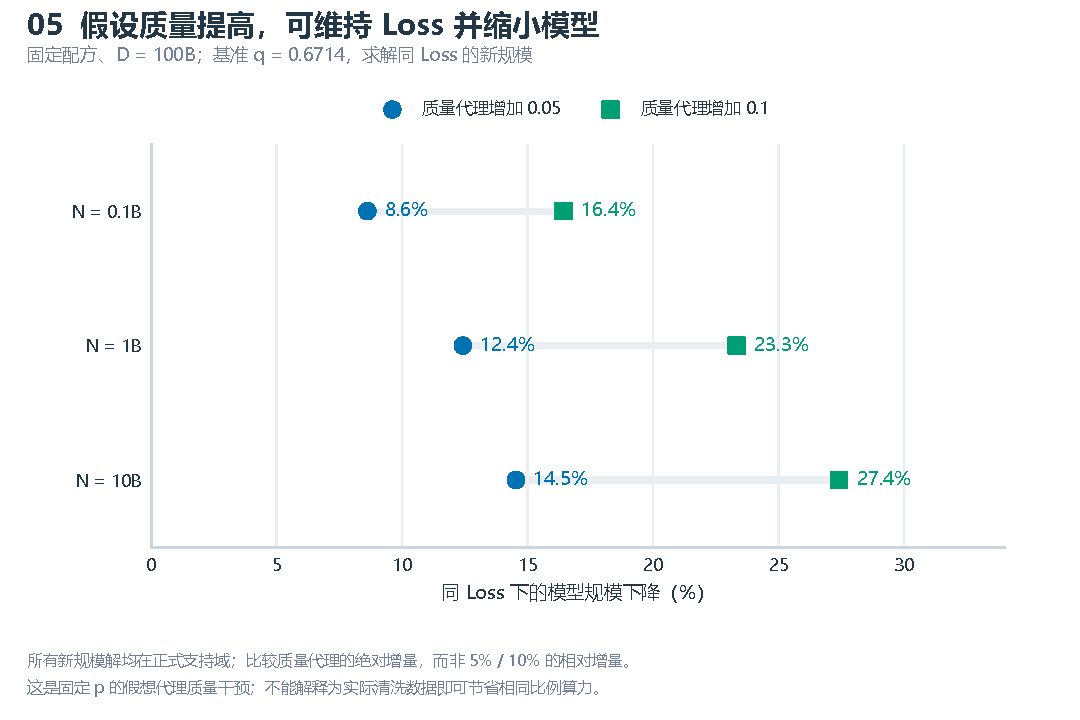
\includegraphics[width=0.89\linewidth]{figures/Q2/05_quality_tradeoff.pdf}
 \caption{固定训练量与配比时，质量提高后维持原 Loss 所需的模型规模变化}
 \label{fig:q2-tradeoff}
\end{figure}

这一计算对应固定配比下的额外质量改善情景。主模型中的 $q(\boldsymbol p)$ 则随配比确定，实际改变训练数据质量时，应同时明确采用的是配比调整还是额外的数据处理。

\subsection{训练领域的替代与互补}

领域配比处于 $\sum_jp_j=1$ 的单纯形上，单独改变一个 $p_j$ 会破坏配比约束。若从训练域 $j$ 向域 $i$ 转移比例 $\epsilon$，即 $\boldsymbol p(\epsilon)=\boldsymbol p+\epsilon(\boldsymbol e_i-\boldsymbol e_j)$，则起点的 Loss 变化率为
\begin{equation}
 \left.\frac{\mathrm d\widehat L}{\mathrm d\epsilon}\right|_{\epsilon=0}
 =\frac{\partial\widehat L}{\partial p_i}
  -\frac{\partial\widehat L}{\partial p_j}.
 \label{eq:q2-transfer}
\end{equation}
在 A4 的平均配比、$N=1$、$D=100$ 及验证域等权的条件下，计算了全部 $\binom{17}{2}=136$ 对领域的局部转移方向，并在 A4 配方凸包内确定可行转移范围。图\ref{fig:q2-transfers}显示，转移效果取决于份额来自哪个领域、流向哪个领域。例如从 FreeLaw 向 arXiv 转移时，起点导数为 $-0.444104$；从 Wikipedia 向 arXiv 转移时为 $-0.769184$，两者都对应起点附近的预测 Loss 下降，但下降幅度不同。

\begin{figure}[htbp]
 \centering
 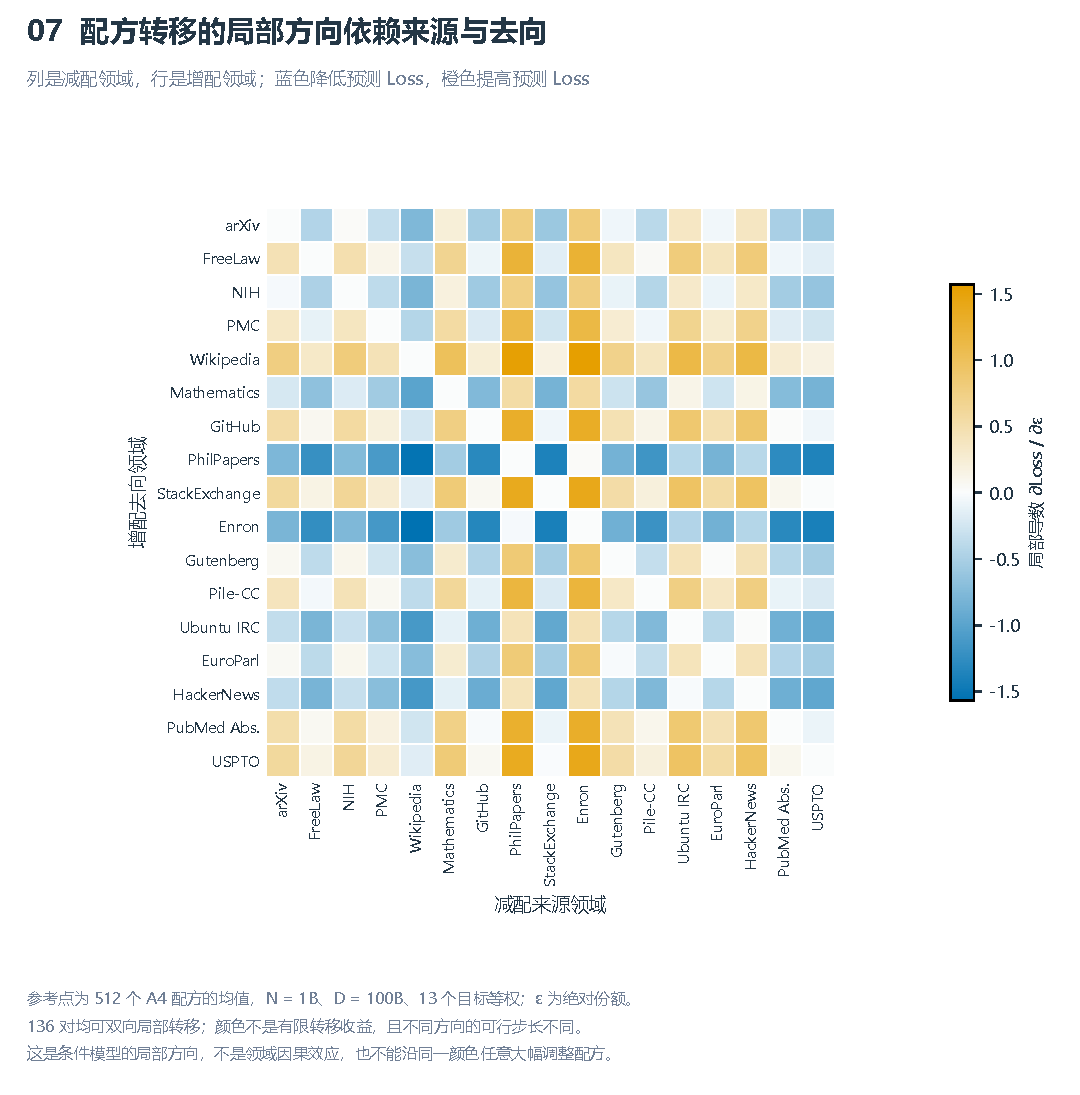
\includegraphics[width=0.94\linewidth]{figures/Q2/07_local_transfers.pdf}
 \caption{平均训练配比附近不同领域间可行转移的局部 Loss 变化方向}
 \label{fig:q2-transfers}
\end{figure}

为比较两个领域联合增加的作用，固定 Pile-CC 作为份额来源，分别从中转出 $\delta$ 给领域 $i$、给领域 $j$，以及同时给两者。令 $\boldsymbol p_i=\boldsymbol p+\delta(\boldsymbol e_i-\boldsymbol e_k)$、$\boldsymbol p_j=\boldsymbol p+\delta(\boldsymbol e_j-\boldsymbol e_k)$、$\boldsymbol p_{ij}=\boldsymbol p+\delta(\boldsymbol e_i+\boldsymbol e_j-2\boldsymbol e_k)$，其中 $k$ 表示 Pile-CC。定义联合效应
\begin{equation}
 I_{ij\mid k}(\delta)
 =\widehat L(\boldsymbol p_{ij})-\widehat L(\boldsymbol p_i)
  -\widehat L(\boldsymbol p_j)+\widehat L(\boldsymbol p),
 \label{eq:q2-pair-effect}
\end{equation}
此处省略固定的 $N,D$ 及验证域权重，计算时质量随配比按式\eqref{eq:q2-quality-map}更新。若 $I_{ij\mid k}<0$，联合增加两域比两次单独增加的 Loss 变化之和更有利，可称为该补偿方式下的互补；$I_{ij\mid k}>0$ 则表现为替代。

取 $\delta=0.005$，Gutenberg 与 EuroParl 的联合效应为 $-1.844\times10^{-5}$，而 arXiv 与 FreeLaw 为 $+1.172\times10^{-5}$，分别呈现互补和替代。前一组在所检验的转移步长及映射强度变化下保持相同符号；后一组的判断会随配比影响强度而变化。这说明领域关系是相对于参考配比、转移方向和份额来源而言的，不能仅凭单个交互系数确定。

\subsection{映射敏感性与结果讨论}

跨来源融合中，第一问质量评分到 B7 质量坐标的映射斜率会影响最终数值。固定配方 172、$N=1$、$D=100$，将式\eqref{eq:q2-quality-map}相对参考质量的斜率分别设为主方案的 0.5、1 和 1.5 倍，得到 $q=0.5534$、$0.6714$、$0.7893$，相应预测 Loss 为 2.3853、2.3443、2.3034，见图\ref{fig:q2-bridge}。这一变化表明，在保持质量排序不变时，映射幅度仍会明显影响 Loss 的计算结果。示例配方中可映射领域占比约为 58.1\%，其余领域仍通过第一问的相对配比效应进入模型。

\begin{figure}[htbp]
 \centering
 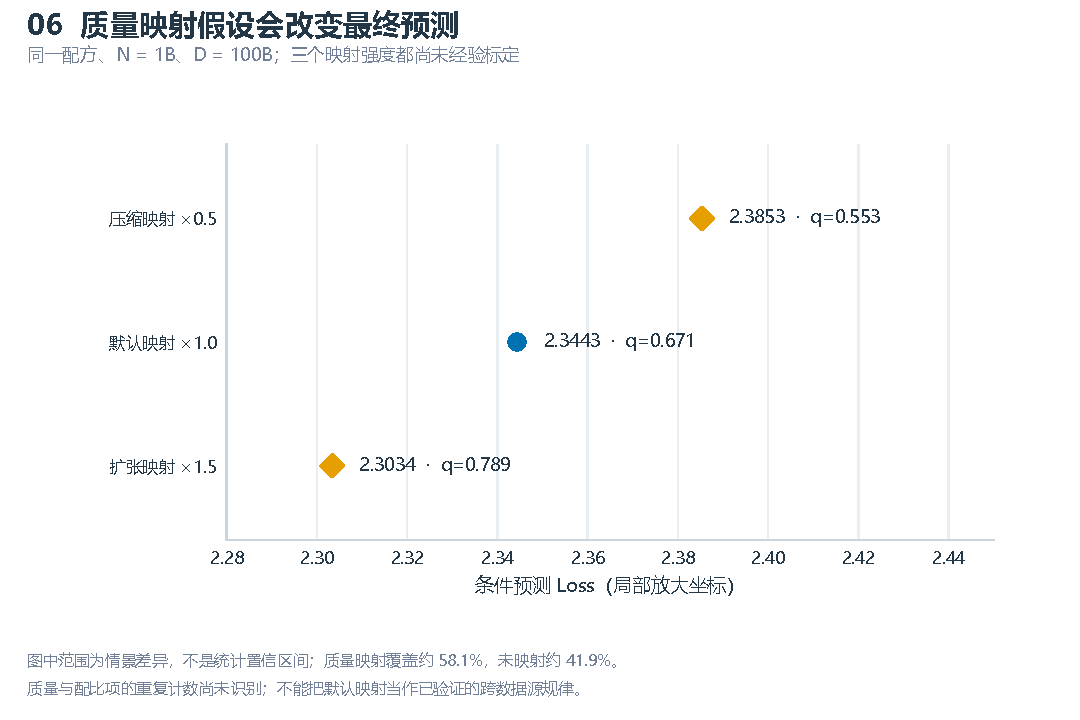
\includegraphics[width=0.88\linewidth]{figures/Q2/06_bridge_sensitivity.pdf}
 \caption{质量评分映射斜率变化对同一训练配方预测 Loss 的影响}
 \label{fig:q2-bridge}
\end{figure}

B9 提供的大模型资料有助于确定外推所涉及的规模量级；B10 的 128 条 Loss 为估算值，其中模型参数量全部超过 B1 的最大值，约 79.7\% 的训练量也超过 B1 上界。虽然估算 Loss 与 B1 曲线的描述性 RMSE 约为 0.00110，两者数值接近仍主要反映估算表的构造关系。因此，B10 用于观察既有函数形式在较大规模下的变化；随着模型规模和数据分布改变，质量映射及配比效应仍需新的成对实验进一步校准。

\subsection{本问结果与后续衔接}

表\ref{tab:q2-output}汇总了本问形成的主要数学量。下一问可以将式\eqref{eq:q2-general}作为给定资源配置下的 Loss 目标，再结合参数训练、数据处理和长文本计算的成本函数比较方案。使用时需同时指定质量变化方式、验证域权重与配比范围：主情景的质量由配比确定；额外提高质量的情景则需为固定配比下的质量变化另计成本。

\begin{table}[htbp]
 \centering\small
 \caption{第二问的主要结果及资源配置中的用途}
 \label{tab:q2-output}
 \begin{tabular}{p{0.21\linewidth}p{0.34\linewidth}p{0.35\linewidth}}
 \toprule
 数学量 & 估计或构造依据 & 后续用途\\
 \midrule
 $L_0(N,D)$ & B1 训练轨迹估计的五参数双幂律 & 计算参数量与训练量变化下的基础 Loss\\
 $G(N,D)$、$q$ & B7 半合成质量项及第一问质量评分的保序映射 & 比较不同质量水平及质量处理投入\\
 $r_{\boldsymbol w}(\boldsymbol p)$ & 第一问的 13 个验证域相对配比效应 & 根据目标偏好评价可行训练配比\\
 $\widehat L$ 及边际量 & 共同范围内的广义标度律与偏导数 & 与算力成本结合，比较资源调整方向\\
 \bottomrule
 \end{tabular}
\end{table}

\subsection{本问小结}

针对跨维度数据融合问题，本文以 B1 建立参数量与训练量的双幂律，再利用 B7 的半合成数据估计随规模变化的质量项，并通过第一问的域级质量评分及相对配比效应构造广义标度律。模型给出了 $N$、$D$、质量与领域配比对 Loss 的局部影响，以及质量提高 0.10 与扩大模型规模之间的定量替代关系。对训练领域的可行转移和联合效应分析表明，领域组合的作用取决于配比调整方式。上述结果为后续在给定算力和数据处理成本下比较资源投入方向提供了数学依据。

% 本章对应赛题问题三。事实依据：仓库 main@f3a49d4 的 Q3 实现、实验与输出。
% 图件由用户提供；N、D 均以十亿为单位。
\setcounter{section}{5}
\section{问题三：算力约束下的多维资源联合优化与结构性转移}
\label{sec:q3}
\setcounter{equation}{0}
\setcounter{figure}{0}
\setcounter{table}{0}

\subsection{问题分析}

在给定算力预算下，增加模型参数量、扩大训练数据量和提高数据质量都会改变验证集交叉熵损失（Loss）\cite{hoffmann2022training,fineweb2024}，同时占用不同的算力。训练领域配比还会改变数据的综合质量和目标域表现。因此，本问需要在同一成本约束下比较这些投入方式，并判断预算增加后最优配置是否发生改变。上下文长度由任务和模型架构决定，本文依据附件 C7 选取 $2048$、$8192$ 和 $131072$ Token 作为外生情景，分别求解资源配置。

第二问已建立参数量 $N$、训练量 $D$、质量和配比到 Loss 的预测关系，可作为本问的目标函数。这里 $N$ 以十亿参数计，$D$ 以十亿 Token 计。第一问的配比观测来自附件 A4，第二问的规模与质量关系分别由 B1 的真实训练记录和 B7 的半合成记录估计。由于附件 A、B 没有同时观测四类因素及同一口径 Loss 的配对实验，本问采用第二问给出的跨来源连接方式，在明确的配比候选范围内求解，并以不同质量机制和假设情景考察结果变化。

表\ref{tab:q3-data-roles}列出各组数据在本问中的作用。B1 与 B7 分别支持规模项和质量项的估计，C7 提供上下文长度的离散情景；附件 A 则提供实际观察过的配比及其相对表现。B7 与 B8 在部分相同坐标上的质量变化趋势不一致，因此本问沿用第二问基于 B7 建立的质量项，不将 B8 混入同一条质量曲线。

\begin{table}[htbp]
 \centering\small
 \caption{问题三所用数据与模型输入的对应关系}
 \label{tab:q3-data-roles}
 \begin{tabular}{lp{4.0cm}p{6.1cm}}
 \toprule
 来源 & 数据性质与规模 & 本问作用\\
 \midrule
 A1、A4、A5 & 质量信号；512 组 17 域配比与 13 个目标域 Loss & 形成配方候选、质量评分及相对配比效应\\
 B1 & 1176 条真实训练记录 & 提供 $N,D$ 双幂标度关系\\
 B7 & 450 条半合成质量记录 & 提供随规模变化的质量项与独立质量情景\\
 C7 & 45 条模型架构元数据 & 选取外生上下文长度，不用于拟合连续注意力成本\\
 \bottomrule
 \end{tabular}
\end{table}

\subsection{资源配置模型}

\subsubsection{预测目标与决策变量}

令 $\boldsymbol p=(p_1,\ldots,p_{17})$ 表示 17 个训练领域的配比，$\sum_i p_i=1$。沿用第二问式\eqref{eq:q2-general}，主方案的预测 Loss 写为
\begin{equation}
 \widehat L(N,D,\boldsymbol p)
 =\left[L_0(N,D)+\{1-q(\boldsymbol p)\}G(N,D)\right]
   \exp\{r_{\boldsymbol w}(\boldsymbol p)\},
 \label{eq:q3-objective}
\end{equation}
其中 $L_0$ 为 B1 的双幂标度律，$G$ 为 B7 的规模相关质量项；$q(\boldsymbol p)$ 由第一问六个可映射领域的质量评分经式\eqref{eq:q2-quality-map}得到，$r_{\boldsymbol w}$ 是第一问 13 个目标域等权平均的相对配比效应。两项都随 $\boldsymbol p$ 改变，因此主方案中的质量不是独立于配比的另一项自由决策。预测采用第二问的共同取值范围
\begin{equation}
 N\in[0.070542,11.965825],\qquad
 D\in[10,299.893],\qquad q\in[0.1,1].
 \label{eq:q3-support}
\end{equation}

配比以 A4 的已观测方案为候选，避免在没有相应实验的连续配比空间中寻优。第一问的无约束配方 136 在本问映射下有 $q\approx0.386$，低于设定的质量基线。本文以满足直接及近似直接质量映射、且 $q(\boldsymbol p)\geq Q_0$ 的 87 个已观测配方组成集合 $\mathcal P$；配方 172 的 $q=0.671361$，作为固定配比对照。令 $Q_0=0.5$，这一基线是本问的情景设定。

\subsubsection{训练、质量与长上下文成本}

依据题面三项成本，将总预算记为 $C_{\max}$，上下文长度记为 $L_{\rm ctx}$。在上述十亿单位下，成本函数为
\begin{align}
 C_{\rm train}&=6\times10^{18}ND,\nonumber\\
 C_{\rm quality}&=10^9D\,[g(q)-g(Q_0)]_+,\nonumber\\
 C_{\rm attn}&=2\times10^{14}NDL_{\rm ctx},\nonumber\\
 C_{\rm total}&=C_{\rm train}+C_{\rm quality}+C_{\rm attn}
                  \leq C_{\max},
 \label{eq:q3-cost}
\end{align}
其中 $[x]_+=\max\{x,0\}$。训练与注意力成本随 $ND$ 增加；质量处理成本还取决于所选配方对应的质量水平。按题面附录 B，分别比较
\begin{equation}
 \begin{aligned}
 g_{\rm exp}(q)&=10^7e^{6q},\\
 g_{\rm pow}(q)&=5\times10^9q^4,\\
 g_{\rm log}(q)&=2\times10^9\ln(1+10q).
 \end{aligned}
 \label{eq:q3-cost-families}
\end{equation}
式\eqref{eq:q3-cost-families}中的 $g$ 表示质量处理的算力成本，与第二问的质量评分映射 $q(\boldsymbol p)$ 含义不同。

综上，对每一组预算、上下文和质量成本形式，求解
\begin{equation}
 \begin{aligned}
 \min_{N,D,\boldsymbol p}\quad &\widehat L(N,D,\boldsymbol p),\\
 \text{s.t.}\quad &C_{\rm total}(N,D,q(\boldsymbol p);L_{\rm ctx})\leq C_{\max},\\
 &\boldsymbol p\in\mathcal P,\quad q(\boldsymbol p)\geq Q_0,\\
 &(N,D,q)\text{ 满足式\eqref{eq:q3-support}}.
 \end{aligned}
 \label{eq:q3-program}
\end{equation}
本文主要考察 $10^{19}$、$10^{22}$、$10^{24}$ FLOPs 三档预算，并增加 $10^{20}$ FLOPs 用于观察过渡过程。

\subsection{模型求解与结构转移识别}

固定一个配方后，$q$ 与配比修正项均为常数。记
$c(L)=6\times10^{18}+2\times10^{14}L$，
$h(q)=10^9[g(q)-g(Q_0)]_+$，成本约束化为
$D\{c(L_{\rm ctx})N+h(q)\}\leq C_{\max}$。
在式\eqref{eq:q3-support}范围内，当前预测模型的 Loss 随 $D$ 增大而下降，故给定 $N$ 时取
\begin{equation}
 D^*(N)=\min\!\left\{D_{\max},
 \frac{C_{\max}}{c(L_{\rm ctx})N+h(q)}\right\},\qquad
 C_{\min}=D_{\min}\{c(L_{\rm ctx})N_{\min}+h(q)\}.
 \label{eq:q3-reduction}
\end{equation}
若 $C_{\max}<C_{\min}$，该配方在给定情景下不可行；否则将式\eqref{eq:q3-reduction}代入目标函数，沿 $\ln N$ 搜索。第二问参数在共同范围内使这一固定配方目标满足所需的分段凸性，因而可比较端点并对导数变号区间二分。对 $\mathcal P$ 中每个可行配方重复求解，最终选择预测 Loss 最小者。这样得到的是 87 个已观测候选中的最优配置。

这一降维过程还便于解释资源取舍。固定配方且质量高于基线时，三种连续变量的边际成本分别为
\begin{equation}
 \frac{\partial C}{\partial N}=c(L_{\rm ctx})D,\qquad
 \frac{\partial C}{\partial D}=c(L_{\rm ctx})N+h(q),\qquad
 \frac{\partial C}{\partial q}=10^9Dg'(q).
 \label{eq:q3-marginal-cost}
\end{equation}
当预算约束起作用且变量处于内部时，单位算力带来的 Loss 下降可由 $-\partial\widehat L/\partial x$ 与相应边际成本之比比较。主方案中 $q=q(\boldsymbol p)$，改变一个领域占比会同时改变质量项与配比项，因此实际求解仍以完整式\eqref{eq:q3-objective}逐配方比较。对于固定配方、可独立提高 $Q_B$ 的方案，则在式\eqref{eq:q3-reduction}的基础上对 $Q_B$ 区间逐段求界并细化，同时检查活跃约束与成本；这使独立质量方案与主方案采用各自一致的变量关系。

为明确“结构性转移”，定义预算 $C$ 下的配置状态为
\begin{equation}
 S(C)=\bigl(I_{\rm feasible}(C),\,j^*(C),\,
 I_{N_{\min}},I_{N_{\max}},I_{D_{\min}},I_{D_{\max}},I_{\rm budget}\bigr),
 \label{eq:q3-state}
\end{equation}
其中 $j^*$ 为最优已观测配方编号，各 $I$ 表示相应约束是否起作用。当可行性、配方或活跃约束改变时，认为资源配置发生结构性转移；单纯的成本占比连续变化不构成新的状态。对每种上下文和成本函数，在 $10^{19}$ 至 $10^{24}$ FLOPs 取 161 个对数等距预算点，随后对相邻异状态点二分定位。固定配方与配比联立的预算扫描共得到 82 个转移括区，其中前者 33 个、后者 49 个。

\subsection{最优配置及成本影响}

\subsubsection{三档预算下的资源选择}

表\ref{tab:q3-config}给出幂函数质量成本下，三档预算与 C7 三种上下文组合的求解结果。低预算时短上下文选择配方 477，训练量处于下界；中预算时配方转为 172，参数量与训练量同步增加。最高预算已达到式\eqref{eq:q3-support}的 $N,D$ 上界，三种上下文因而得到相同的预测 Loss。图\ref{fig:q3-configuration}概括了这一变化。

\begin{table}[htbp]
 \centering\small
 \caption{幂函数质量成本下的配比联立配置（$N,D$ 为十亿单位）}
 \label{tab:q3-config}
 \begin{tabular}{rrrrrrr}
 \toprule
 预算/FLOPs & 上下文/Token & 配方 & $N$ & $D$ & $q$ & 预测 Loss\\
 \midrule
 $10^{19}$ & 2048 & 477 & 0.104 & 10.000 & 0.600 & 3.1551\\
 $10^{19}$ & 8192 & 477 & 0.087 & 10.000 & 0.600 & 3.2038\\
 $10^{19}$ & 131072 & \multicolumn{5}{c}{共同取值范围内不可行}\\
 $10^{22}$ & 2048 & 172 & 7.291 & 210.799 & 0.671 & 2.0809\\
 $10^{22}$ & 8192 & 172 & 6.661 & 193.874 & 0.671 & 2.0944\\
 $10^{22}$ & 131072 & 172 & 3.214 & 95.943 & 0.671 & 2.2179\\
 $10^{24}$ & 2048 & 172 & 11.966 & 299.893 & 0.671 & 2.0195\\
 $10^{24}$ & 8192 & 172 & 11.966 & 299.893 & 0.671 & 2.0195\\
 $10^{24}$ & 131072 & 172 & 11.966 & 299.893 & 0.671 & 2.0195\\
 \bottomrule
 \end{tabular}
\end{table}

\begin{figure}[htbp]
 \centering
 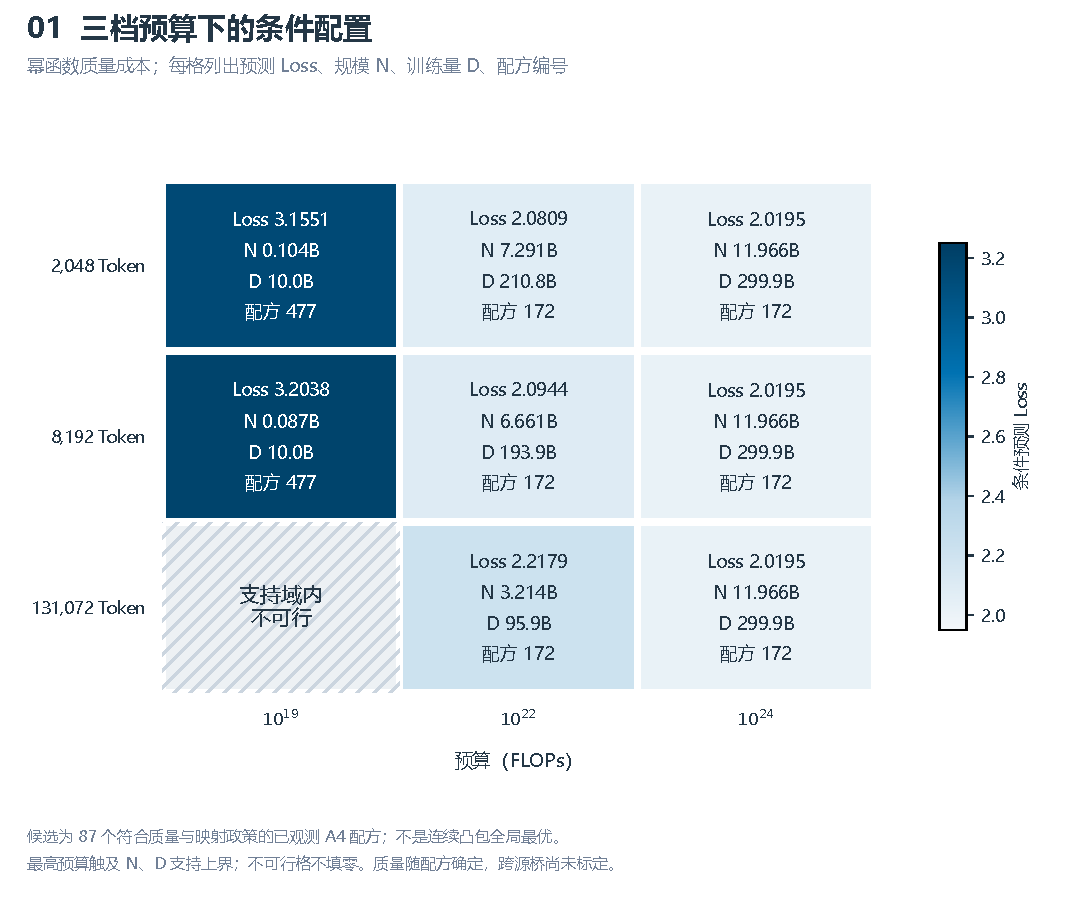
\includegraphics[width=0.86\linewidth]{figures/Q3/01_configuration.pdf}
 \caption{三档预算与三种上下文下的配比联立配置}
 \label{fig:q3-configuration}
\end{figure}

固定配方 172 的 36 个预算、上下文和成本函数组合中有 30 个可行；允许在 87 个配方中选择后，可行组合增至 33 个。这说明配比调整在低预算下不仅改变 Loss，也能够通过改变质量成本使某些配置进入可行范围。在 8192 Token、幂成本下，最优配方于 $[1.610535,1.610648]\times10^{19}$ FLOPs 内由 477 切换为 172，见图\ref{fig:q3-switch}。低预算阶段，质量成本较低的配方有利于满足预算；预算放宽后，配方 172 的综合预测表现占优。

预算扫描的分辨率会影响短暂状态的识别。将每组扫描由 81 点加密至 161 点后，131072 Token 情景在可行性边缘出现若干短暂配方状态；粗网格会漏过它们。故本文以加密扫描及二分得到的预算区间报告转移位置，不将图\ref{fig:q3-switch}中的切换推广为所有上下文下的唯一转移。

\begin{figure}[htbp]
 \centering
 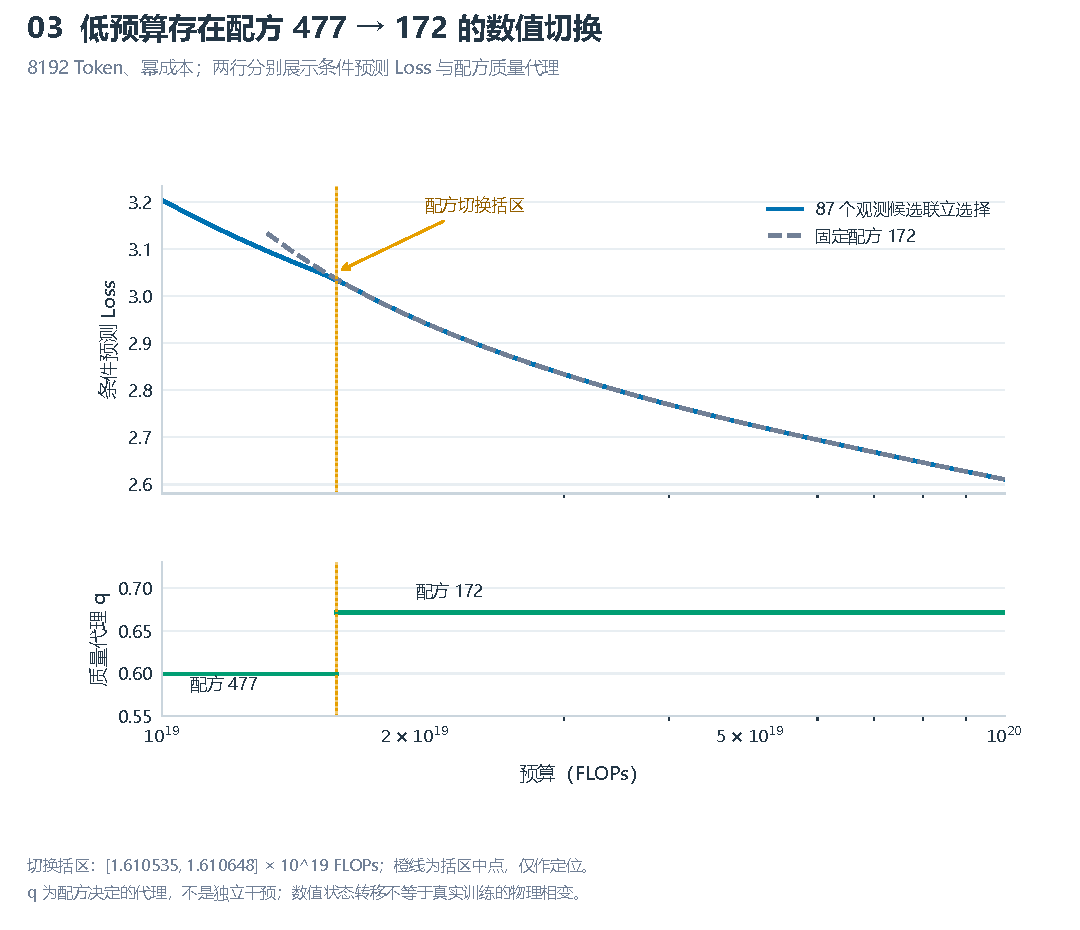
\includegraphics[width=0.84\linewidth]{figures/Q3/03_recipe_switch.pdf}
 \caption{8192 Token、幂函数成本下最优配方的预算切换}
 \label{fig:q3-switch}
\end{figure}

\subsubsection{质量成本形式与预算分解}

质量成本函数改变了低预算时各配方的相对代价。8192 Token、$10^{19}$ FLOPs 下，指数成本选配方 172，预测 Loss 为 3.12884；幂函数和对数成本均选配方 477，Loss 分别为 3.20379 和 3.19274。到 $10^{22}$ FLOPs，三种函数均选配方 172，Loss 依次为 2.09389、2.09442 和 2.09411。图\ref{fig:q3-families}以各预算自身的局部坐标显示这一差异。可见成本形式主要影响低预算的配方选择；在中预算时，方案趋于一致。

\begin{figure}[htbp]
 \centering
 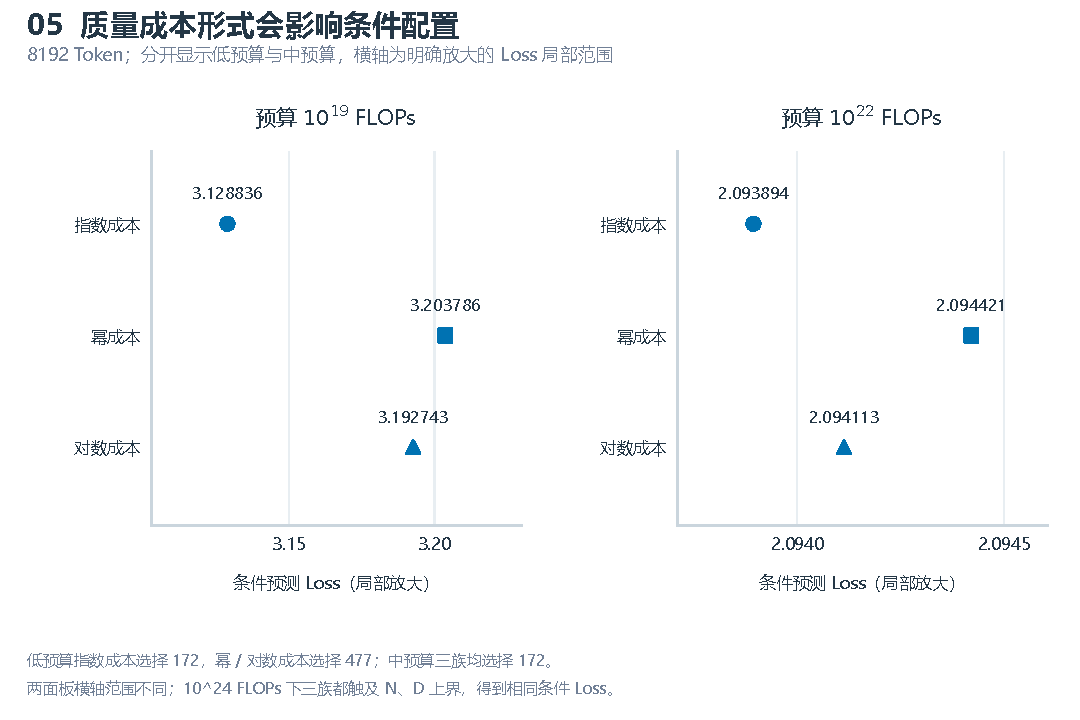
\includegraphics[width=0.84\linewidth]{figures/Q3/05_cost_families.pdf}
 \caption{不同质量成本函数对低、中预算配置的影响}
 \label{fig:q3-families}
\end{figure}

图\ref{fig:q3-cost-allocation}将预算分为基础训练、注意力、质量处理和未使用部分。$10^{19}$ 与 $10^{22}$ FLOPs 的可行最优配置基本用满预算，而 $10^{24}$ FLOPs 时，幂成本下三个上下文的使用率分别为 2.32\%、2.76\% 和 11.58\%。原因在于 $N,D$ 已达到共同数据范围上界；这一平台反映模型的取值范围，而非更大训练配置的收益必然消失。

表\ref{tab:q3-cost-shares}从中选取 8192 Token 的三档预算，列出与表\ref{tab:q3-config}对应的成本分解。低预算中质量处理占 33.3\%，中预算降至 1.4\%，基础训练和注意力开销成为主要部分；高预算的未使用比例达到 97.2\%，与变量触及支持上界相一致。表中各项均以对应预算为分母，便于直接比较资源去向。

\begin{table}[htbp]
 \centering\small
 \caption{8192 Token、幂函数成本下的预算分解（占预算的百分比）}
 \label{tab:q3-cost-shares}
 \begin{tabular}{rrrrr}
 \toprule
 预算/FLOPs & 基础训练 & 注意力 & 质量处理 & 未使用\\
 \midrule
 $10^{19}$ & 52.36\% & 14.30\% & 33.34\% & 0.00\%\\
 $10^{22}$ & 77.48\% & 21.16\% & 1.36\% & 0.00\%\\
 $10^{24}$ & 2.15\% & 0.59\% & 0.02\% & 97.24\%\\
 \bottomrule
 \end{tabular}
\end{table}

\begin{figure}[htbp]
 \centering
 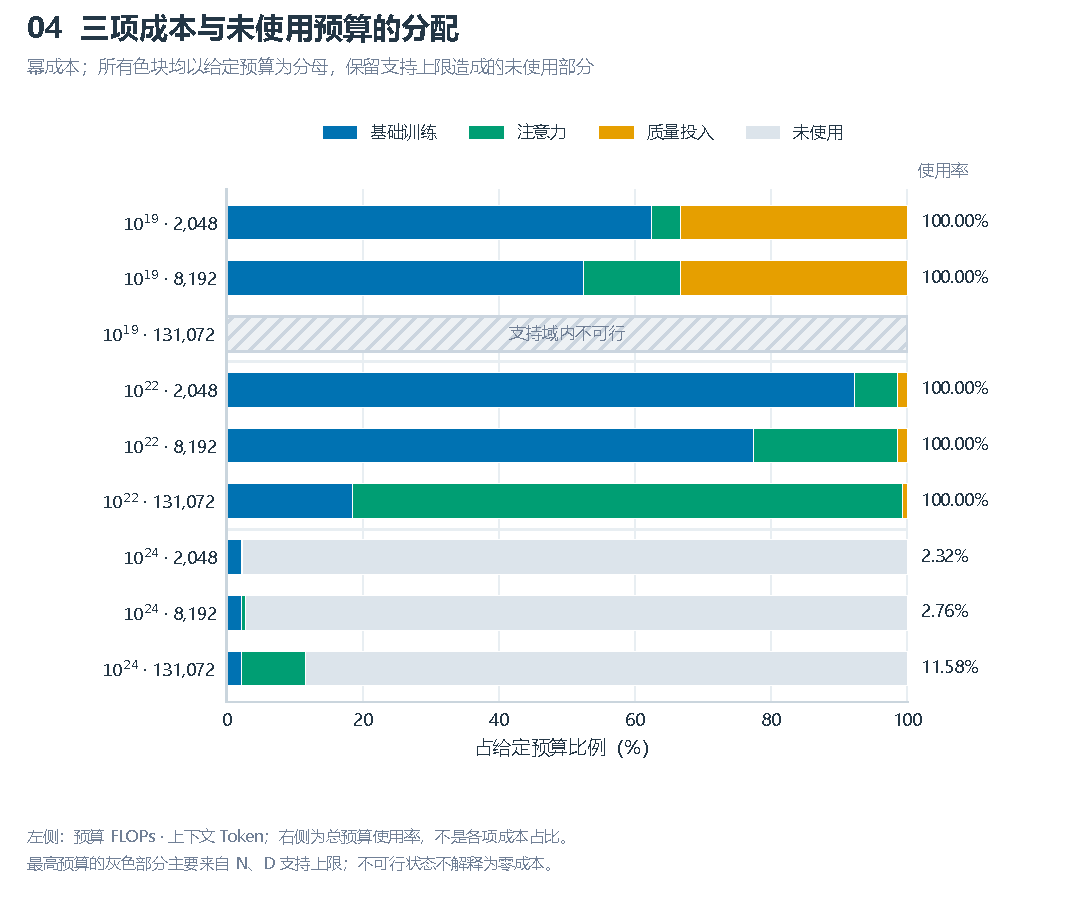
\includegraphics[width=0.86\linewidth]{figures/Q3/04_cost_allocation.pdf}
 \caption{幂函数质量成本下三项开销及未使用预算的比例}
 \label{fig:q3-cost-allocation}
\end{figure}

\subsection{上下文长度与独立质量投入}

\subsubsection{长上下文的临界长度}

由式\eqref{eq:q3-cost}可直接得到
\begin{equation}
 \frac{C_{\rm attn}}{C_{\rm train}}
 =\frac{2\times10^{14}L_{\rm ctx}}{6\times10^{18}}
 =\frac{L_{\rm ctx}}{30000},\qquad
 L_{\rm ctx}^{\rm crit}=30000\ \text{Token}.
 \label{eq:q3-context-critical}
\end{equation}
因此，C7 的 2048、8192、131072 Token 三种情景下，注意力与基础训练成本之比分别为 0.0683、0.2731 和 4.3691。图\ref{fig:q3-context}给出了代数关系。在中预算、幂成本下，将上下文由 2048 延长至 131072 Token，最优 $N$ 从 7.291 降至 3.214，$D$ 从 210.799 降至 95.943，预测 Loss 从 2.0809 升至 2.2179。长上下文直接挤占可分配给规模与训练量的预算\cite{flashattention2022}；低预算的最长上下文则在共同取值范围内不可行。临界长度描述两项成本相等的位置，131072 Token 情景在 C7 中的观测支持较稀疏。

\begin{figure}[htbp]
 \centering
 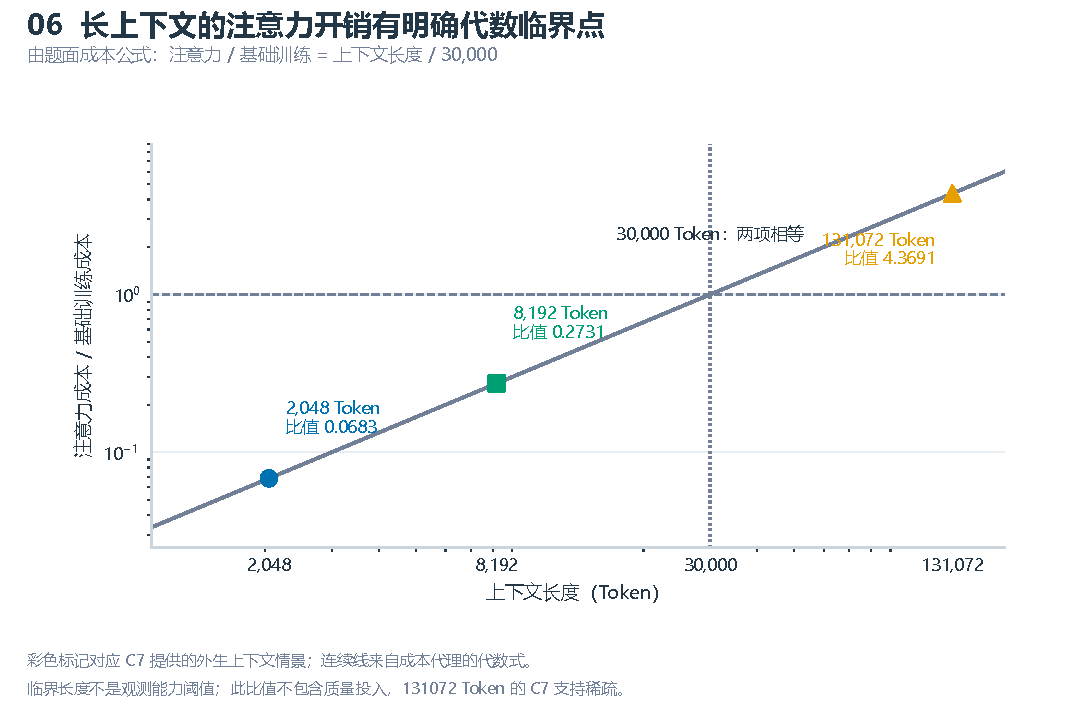
\includegraphics[width=0.84\linewidth]{figures/Q3/06_context_cost.pdf}
 \caption{上下文长度与注意力成本相对基础训练成本的关系}
 \label{fig:q3-context}
\end{figure}

\subsubsection{固定配比下的独立质量选择}

主模型通过改变配比影响质量。为考察另一种投入方式，再固定配方 172，把 B7 中的质量坐标 $Q_B\in[Q_0,1]$ 作为可独立提高的变量，以式\eqref{eq:q3-cost}计入相应成本。此时目标为 $[L_0(N,D)+(1-Q_B)G(N,D)]\exp\{r_{\boldsymbol w}(\boldsymbol p_{172})\}$，联合选择 $N,D,Q_B$。在 8192 Token、幂成本下，结果如表\ref{tab:q3-independent}及图\ref{fig:q3-independent}所示。

\begin{table}[htbp]
 \centering\small
 \caption{固定配方 172、独立提高质量时的配置（8192 Token，幂成本）}
 \label{tab:q3-independent}
 \begin{tabular}{rrrrrl}
 \toprule
 预算/FLOPs & $N$ & $D$ & $Q_B$ & 预测 Loss & 主要配置特征\\
 \midrule
 $10^{19}$ & 0.1309 & 10.000 & 0.500 & 3.0969 & 质量处于基线\\
 $10^{20}$ & 0.7628 & 10.000 & 0.973 & 2.5618 & 训练量仍在下界\\
 $10^{22}$ & 5.2587 & 222.936 & 1.000 & 2.0232 & 质量达到上界\\
 $10^{24}$ & 11.9658 & 299.893 & 1.000 & 1.9570 & 三项达到上界\\
 \bottomrule
 \end{tabular}
\end{table}

低预算下先满足最低训练量，质量保持在 $Q_0$；预算升至 $10^{20}$ FLOPs 时，质量提高而训练量仍为 10；中预算时，质量达到上界且训练量显著增加。这展示了允许独立质量处理后，不同资源进入最优配置的先后次序。该方案以质量处理能够改变 B7 质量坐标为前提，与主方案的“配比决定质量”对应不同的投入机制。

进一步扫描独立质量方案的预算，得到两个约束状态的转换区间：
\begin{align}
 Q_B\text{ 离开基线：}\quad
 C&\in[1.228876,1.228962]\times10^{19}\ \text{FLOPs},\nonumber\\
 Q_B\text{ 接近上界：}\quad
 C&\in[1.085995,1.086071]\times10^{20}\ \text{FLOPs}.
 \label{eq:q3-native-transitions}
\end{align}
这两个区间解释了表\ref{tab:q3-independent}中质量先保持基线、再快速增加、最终达到上界的过程。将求解精度提高一个数量级后，区间两侧的质量状态保持一致；区间位置仍由 B7 的半合成质量关系和所选成本函数决定。

\begin{figure}[htbp]
 \centering
 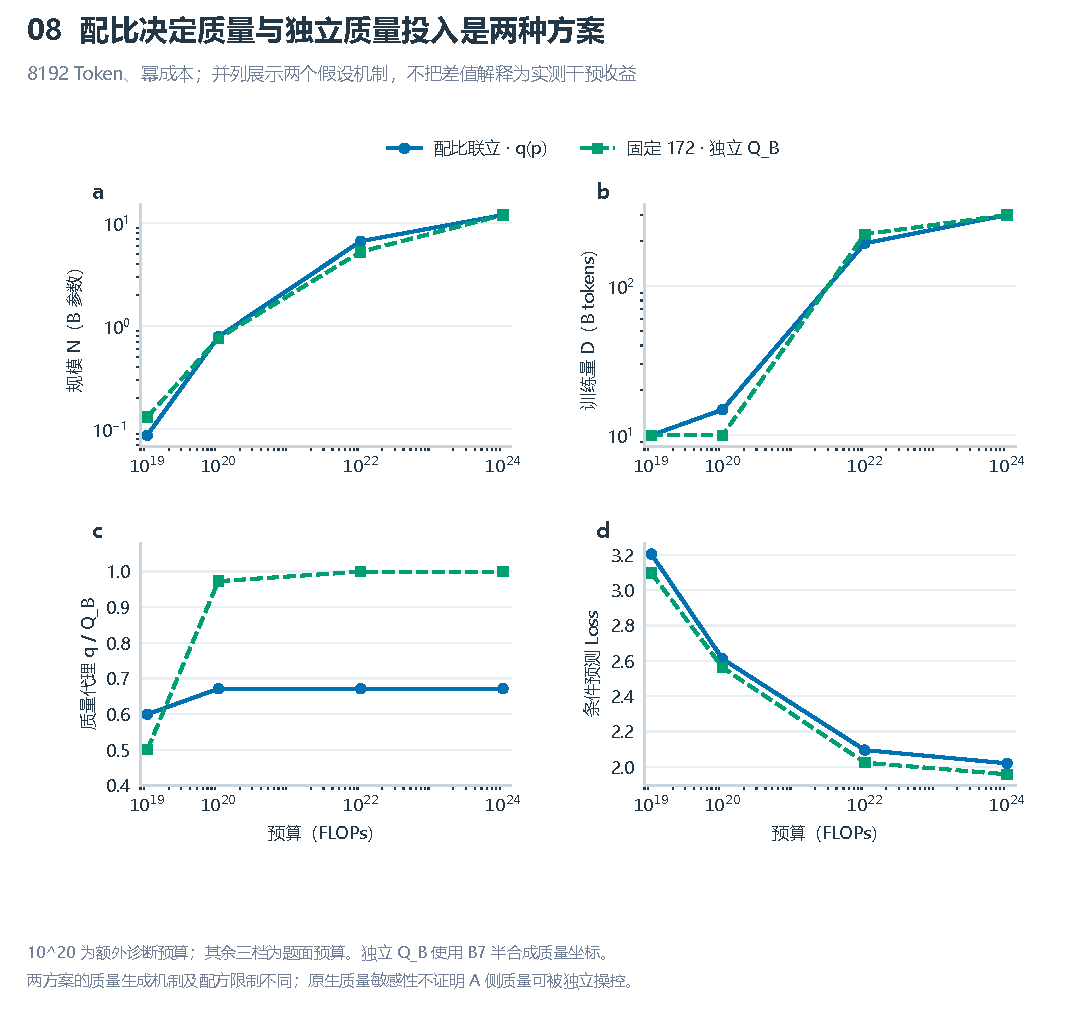
\includegraphics[width=0.86\linewidth]{figures/Q3/08_independent_quality.pdf}
 \caption{配比决定质量与固定配比下独立质量投入的配置轨迹}
 \label{fig:q3-independent}
\end{figure}

\subsection{假设敏感性与模型检验}

\subsubsection{配方选择的敏感性}

第一问质量评分与 B7 质量坐标的连接、基线质量及配比效应幅度都会影响成本和预测 Loss。为检验选择的稳定性，分别改变 $Q_0$、质量映射斜率倍数 $s$ 和配比效应倍数 $\lambda$，其余条件保持主情景。图\ref{fig:q3-assumptions}汇总九种单因素情景在三档预算、三种上下文和三类成本函数组成的 27 个格上的结果。

\begin{figure}[htbp]
 \centering
 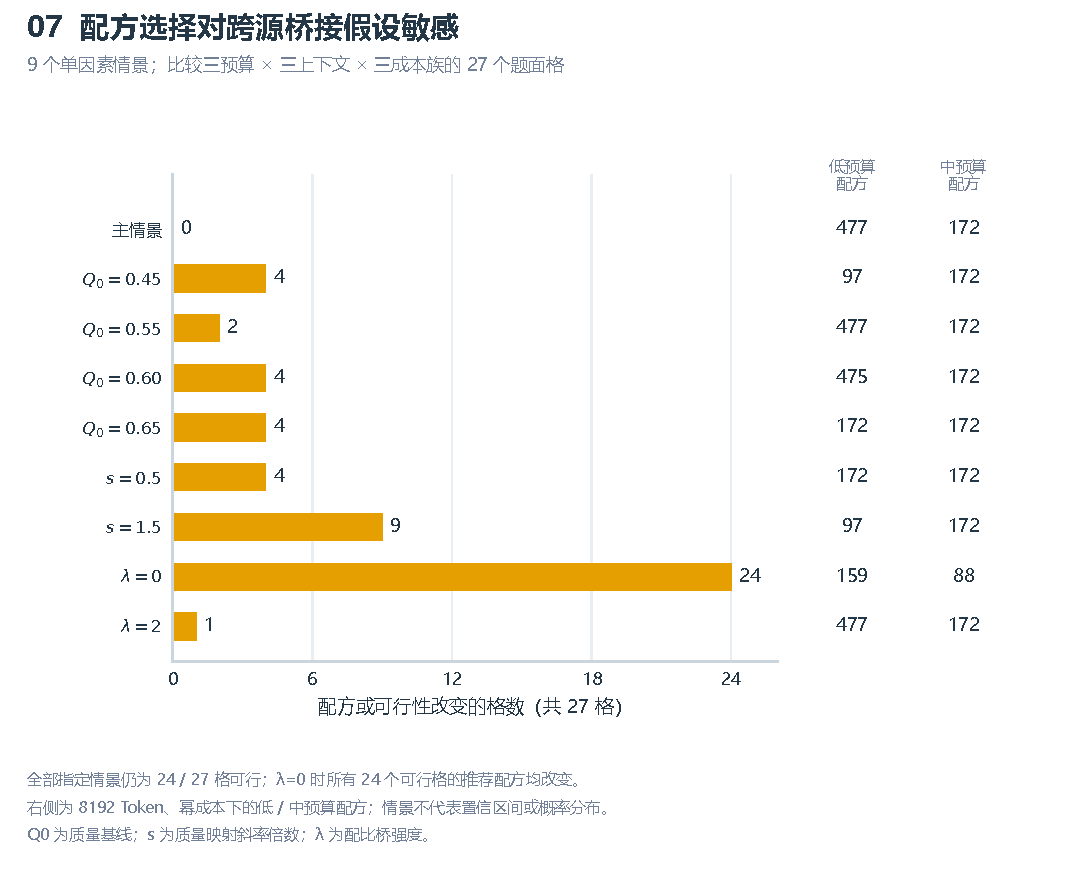
\includegraphics[width=0.86\linewidth]{figures/Q3/07_assumptions.pdf}
 \caption{质量基线、评分映射与配比效应变化对最优配方的影响}
 \label{fig:q3-assumptions}
\end{figure}

各情景均有 24 个格可行，但低预算配方对假设较敏感。主情景在 8192 Token、幂成本下选 477；当 $Q_0=0.60$ 时，由于配方 477 的质量约为 0.599515，方案改为 475；$Q_0=0.65$ 时改为 172。将配比效应设为零，即 $\lambda=0$，27 格中的 24 个可行格均改变所选配方。这表明预算及成本约束决定可行范围，而配比效应的设定对配方排序具有较大影响。

配方切换的预算位置也随假设改变：$Q_0=0.55$ 时，上述 8192 Token、幂成本下的 $477\to172$ 切换提前至约 $[1.46552,1.46560]\times10^{19}$ FLOPs；将配比效应倍数设为 $\lambda=2$ 时，进一步提前至约 $[1.28214,1.28221]\times10^{19}$ FLOPs。质量映射斜率增至 1.5 倍时，低预算先选择 97，再经历 97、477、172 的连续切换。由此可见，中预算配方在多数情景下相对稳定，低预算的配方编号与切换点则需要随质量映射假设一同报告。

\subsubsection{数值求解的复算}

对固定配方、配比联立和独立质量三种方案，分别在 36 个预算、上下文和成本函数组合上独立复算。三组可行状态数为 30、33、33；复算所得的可行性与配方选择均一致，预测 Loss 的最大差低于 $10^{-12}$。这支持了降维求解与独立质量搜索的数值一致性。

\subsubsection{外部实验的排序检验}

进一步利用公开的 OpenLM 训练记录\cite{gadre2024}\footnote{公开模型与评测记录见 \url{https://github.com/mlfoundations/scaling}。}检验规模项的排序能力。104 个实际训练模型中，42 个落在本问 $N,D$ 的共同范围内；按 C4、RedPajama 和 RefinedWeb 三种训练语料各取 14 个，用同一 Paloma C4 验证集的观测 Loss 比较 B1 规模模型的预测排序。图\ref{fig:q3-external}中，三个语料组的 Spearman 相关系数依次为 0.9736、0.9868 和 0.9736。在使预算真正筛除部分候选的 6 组离散选择中，按规模模型选出的方案有 5 组与最低观测 Loss 一致；RefinedWeb 的 $10^{21}$ FLOPs 组未命中，观测 Loss 差为 0.0705。

\begin{figure}[htbp]
 \centering
 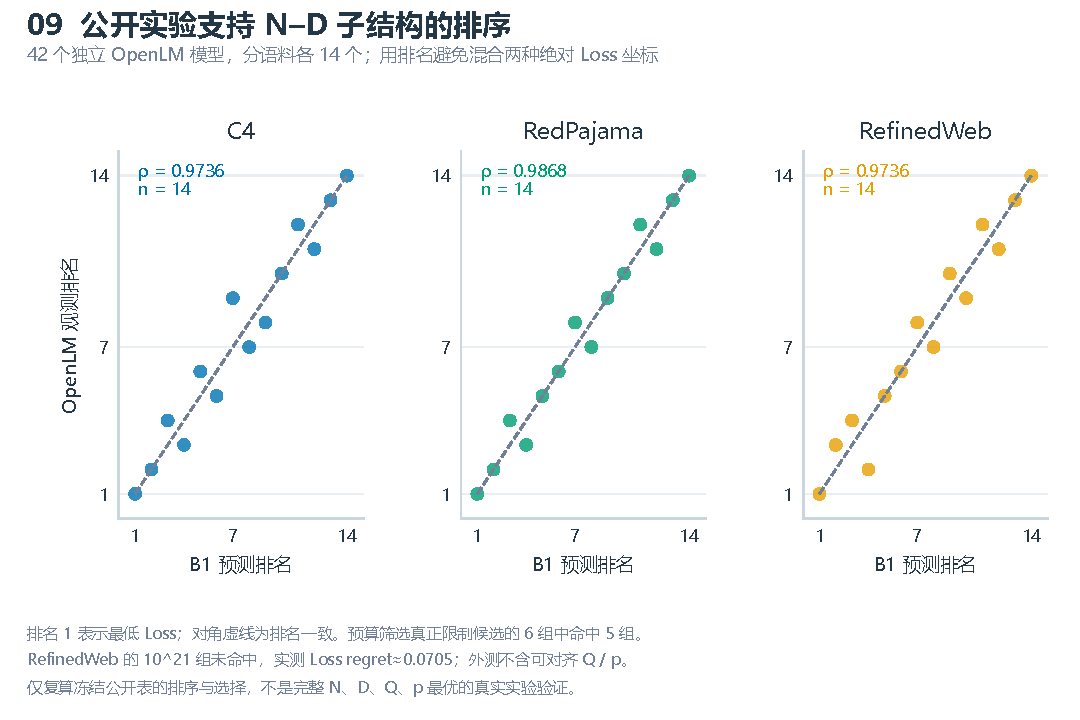
\includegraphics[width=0.86\linewidth]{figures/Q3/09_external_ranks.pdf}
 \caption{公开训练模型中参数量与训练量预测排序的外部检验}
 \label{fig:q3-external}
\end{figure}

这一检验表明 $N,D$ 规模关系在独立训练记录中保持了较好的相对排序，也揭示了个别预算组的选择偏差。公开记录没有与本问 17 域配比及质量评分相对应的观测量，因此配方及独立质量投入的数值仍应结合新的联合训练实验进一步校准。

\clearpage
\subsection{本问输出与后续衔接}

表\ref{tab:q3-output}汇总本问向后续能力分析提供的三类配置。每一行方案均包含预算、上下文、成本形式、可行状态、所选 $N,D$、配方或质量坐标、三项成本及预测 Loss。固定配方与配比联立使用由配比决定的 $q(\boldsymbol p)$；独立质量方案使用 B7 的 $Q_B$，两种质量坐标在后续分析中需保持区分。问题四若将这些配置与能力指标联系，还需处理不同验证 Loss 与评测分数之间的映射；本问的预算解本身提供的是资源配置和相应的条件 Loss。

\begin{table}[htbp]
 \centering\small
 \caption{问题三的配置结果及其后续用途}
 \label{tab:q3-output}
 \begin{tabular}{lp{4.0cm}cp{5.0cm}}
 \toprule
 方案 & 决策变量 & 可行格数 & 输出含义\\
 \midrule
 固定配方 172 & $N,D$；$q(\boldsymbol p_{172})$ 固定 & 30/36 & 比较预算、上下文与成本形式的规模选择\\
 已观测配方联立 & $N,D,\boldsymbol p\in\mathcal P$；$q$ 随配比变化 & 33/36 & 给出 87 个候选中的配方与规模配置\\
 独立质量投入 & $N,D,Q_B$；配方 172 固定 & 33/36 & 比较单独提高质量时的资源分配次序\\
 \bottomrule
 \end{tabular}
\end{table}

\subsection{本问小结}

本问将第二问的广义标度律与训练、质量处理和长上下文三项成本结合，在三个数量级的算力预算下求得配比、模型规模和训练量的配置。幂成本主情景显示：低预算选择配方 477 并维持最低训练量；中预算转向配方 172，同时扩展 $N,D$；高预算达到现有数据的共同支持上界。质量成本形式影响低预算的配方选择；上下文达到 30000 Token 时，注意力成本与基础训练成本相当。独立质量投入方案还揭示了从质量基线到质量上界的两个预算转移。重复求解、假设敏感性和公开模型的排序检验共同说明了数值配置的稳定部分与对跨来源假设较敏感的部分，为后续能力分析提供了带有明确变量口径的资源方案。

% 本章对应赛题问题四。事实依据：仓库 main@f3a49d4 的 Q4 实现、实验与输出。
% 图件由用户提供；所列未来月份均从附件中的最后提交日期起算。
\setcounter{section}{6}
\section{问题四：技术演进分析与前沿预测}
\label{sec:q4}
\setcounter{equation}{0}
\setcounter{figure}{0}
\setcounter{table}{0}

\subsection{问题分析与数据整理}

本问需要回答两个相互关联的问题：历史能力增长中，模型规模变化与同规模条件下的变化分别占多少；若算力增速放缓，未来一至两年开源模型的高端能力和最高能力可能达到什么水平。前三问以交叉熵 Loss 度量模型表现，而本问以多项 Benchmark 得分度量能力，因此还需建立来源一致的 Loss--能力关系\cite{gadre2024,observational2024}，分析前述配置在能力坐标上的含义。

令模型 $i$ 的综合能力为 C2 六项得分的等权均值
\begin{equation}
 S_i=\frac{1}{6}\sum_{k=1}^{6}s_{ik},\qquad 0\leq S_i\leq100,
 \label{eq:q4-score}
\end{equation}
六项分别为 IFEval、BBH、MATH Lvl 5、GPQA、MUSR 和 MMLU-PRO\cite{mmlupro2024}。仅当六项均有有效得分时计算 $S_i$。时间轴采用榜单提交日；模型类型分为基础预训练和后训练两组，后者包含 chat 与领域微调。开放模型筛选排除明确标注不开放权重的记录，并结合权重及许可证标签；严格开放和许可证口径另作敏感性比较。许可证标签只能作为开放可用性的筛选依据，具体研究与复现权限仍由对应许可证决定。对同名模型在当期分析中保留最新提交版本，但计算历次最高分时保留所有历史版本。

表\ref{tab:q4-data}概括本问的数据角色。C2 去重后的扩展开放集合为 2616 个模型，其中主分析使用基础预训练 204 个、后训练 1620 个。C3 的 4599 行记录来自不同评分来源和年份；其中历史报告的 26 行原有 Average 与式\eqref{eq:q4-score}所算六任务均值的平均绝对差为 9.101 分，因此按来源、年份和任务分别分析，不把不同口径的 Average 拼接成同一能力曲线。C8 的 1860 个可解析模型均有 24 项 BBH 任务结果。逐模型聚合后，BBH 宏平均的中位数为 49.40 分，而任务最低分的中位数为 14 分，1368 个模型至少有一项任务低于 20 分，说明综合均分会掩盖任务短板。C7 提供 2048、8192 和 131072 Token 三档已观察到的上下文长度，作为与第三问衔接的配置情景；最高一档仅有一个对应模型，不用于估计上下文长度的独立能力效应。

\begin{table}[htbp]
 \centering\small
 \caption{问题四的数据来源与分析用途}
 \label{tab:q4-data}
 \begin{tabular}{lp{4.0cm}p{6.4cm}}
 \toprule
 来源 & 数据性质 & 本问用途\\
 \midrule
 C2 & 六项能力得分、类型、提交日、开放标签 & 定义能力、历史分解、前沿回测及预测\\
 C3 & 多来源历史能力记录 & 分来源和逐任务考察长期变化，核对评分口径\\
 C4 & 参数量、训练量、算力与开放权重信息 & 估计资源增长情景并比较筛选口径\\
 C6 & Loss 与能力的成对记录 & 在各自来源内建立 Loss--能力关系\\
 C7 & 模型架构及上下文长度记录 & 确定跨问题配置所用的上下文情景\\
 C8 & BBH 原始逐任务结果 & 检查任务分布与均分掩盖的短板\\
 \bottomrule
 \end{tabular}
\end{table}

在 C3 的同一现代榜单来源内，2024 年和截至附件截点的 2025 年提交样本，六任务均分的第 90 百分位分别为 35.108 和 39.665 分；其中 MATH Lvl 5 的单任务第 90 百分位由 32.175 升至 45.846 分。按上述重复键去重后，两年六任务第 90 百分位为 35.100 和 39.626 分，变化很小。历史论文报告组则存在较高的任务零值比例与不同的 Average 口径，故它用于观察各项任务的历史覆盖和得分差异，不与现代榜单直接拼接预测。

C4 的 3523 条资源记录中，$N,C,D$ 均为正且有限的有 850 条。进一步按生成式语言任务、显式开放权重、Token 单位、基础模型、架构和来源可靠性筛选，并以 $C/(6\times10^{18}ND)\in[0.5,2]$ 检查资源单位的一致性，得到主集合 81 条；将最后一项放宽为 $[0.1,10]$，得到 93 条。这里 $N,D$ 分别以十亿参数和十亿 Token 计，$C$ 为 FLOPs。计算量有些本就由 $N,D$ 估算，因此上述比值用于核对口径。对 2021--2024 年各年算力的第 90 百分位取常用对数并拟合年度趋势，主集合的年增速为 $g_C=0.690315$ 个十进对数单位，即年倍率约 4.901；放宽集合分别为 0.600552 和 3.986。图\ref{fig:q4-resources}显示两种筛选下的资源变化。后续把这些速率作为未来投入情景，不直接解释为能力增长的因果系数。

\begin{figure}[htbp]
 \centering
 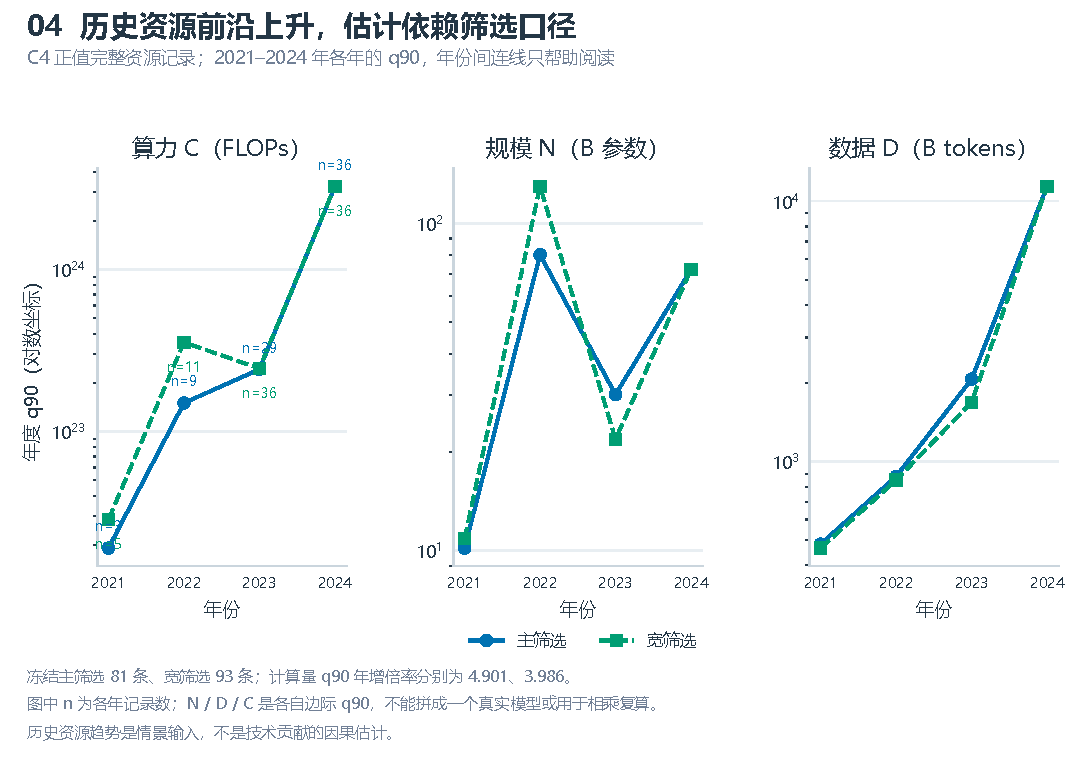
\includegraphics[width=0.84\linewidth]{figures/Q4/04_resources.pdf}
 \caption{两种筛选口径下的历史算力、参数量和训练量上沿}
 \label{fig:q4-resources}
\end{figure}

\subsection{历史能力变化的标准化分解}

\subsubsection{规模分布与同格变化}

为比较规模扩张和其余变化，在相同模型类型内分别取最早与最晚的两个月样本，按 $\log_{10}N$ 划分参数格，要求每格两期均至少有两个模型。后训练组中的 chat 与领域微调先分别处理，再使用两期合并样本形成固定类型权重 $\pi_g$。设 $w_{gjt}$ 为类型 $g$ 内参数格 $j$ 在时期 $t$ 的样本权重，$m_{gjt}$ 为该格能力均值，定义共同支持上的标准化均值 $M_t=\sum_g\pi_g\sum_jw_{gjt}m_{gjt}$。对 $M_1-M_0$ 作对称分解：
\begin{align}
 \Delta_{\rm scale}
 &=\frac12\sum_g\pi_g\sum_j(w_{gj1}-w_{gj0})(m_{gj1}+m_{gj0}),
 \label{eq:q4-scale-term}\\
 \Delta_{\rm within}
 &=\frac12\sum_g\pi_g\sum_j(w_{gj1}+w_{gj0})(m_{gj1}-m_{gj0}),
 \label{eq:q4-within-term}\\
 \Delta_{\rm std}&=M_1-M_0=\Delta_{\rm scale}+\Delta_{\rm within},\nonumber\\
 \Delta_{\rm gap}&=\Delta_{\rm full}-\Delta_{\rm std}.
 \label{eq:q4-gap}
\end{align}
第一项衡量样本在参数格间移动所造成的均分变化，第二项衡量相同格内的变化；全样本与共同支持结果之差单独留在 $\Delta_{\rm gap}$。这一恒等式避免将样本组成和支持范围变化误计入某一贡献。

表\ref{tab:q4-decomp}给出 $0.5$ decade 参数格的主结果。后训练组的共同支持均分由 18.937 升至 24.700，增量 5.763 分；参数分布项为 $-0.758$ 分，同格变化为 $6.521$ 分。相对标准化增量，两项带符号份额分别为 $-13.15\%$ 和 $113.15\%$。超过 100\% 的份额源于规模分布项的反向抵消。若假定同格内训练量、后训练投入和评测选择近似稳定，可将前者视为可见规模变化的贡献，后者视为非规模变化的剩余贡献。附件缺少与 C2 逐模型对齐的 $D$ 及训练过程信息，故同格项也可能包含数据量、后训练和样本选择的变化。基础组的标准化增量仅 0.880 分，其比例对小分母较敏感，表中保留分值而不汇总总体百分比。图\ref{fig:q4-contributions}直观展示三项如何组成全样本增量。

\begin{table}[htbp]
 \centering\small
 \caption{两月窗口、$0.5$ decade 参数格下的能力变化分解（分）}
 \label{tab:q4-decomp}
 \begin{tabular}{lrrrrrr}
 \toprule
 类型 & 共同支持早/晚 & 标准化变化 & 参数分布 & 同格变化 & 支持差 & 全样本变化\\
 \midrule
 后训练 & 313/423 & 5.763 & $-0.758$ & 6.521 & $-1.542$ & 4.222\\
 基础预训练 & 78/41 & 0.880 & $-3.756$ & 4.636 & $-2.072$ & $-1.192$\\
 \bottomrule
 \end{tabular}
\end{table}

\begin{figure}[htbp]
 \centering
 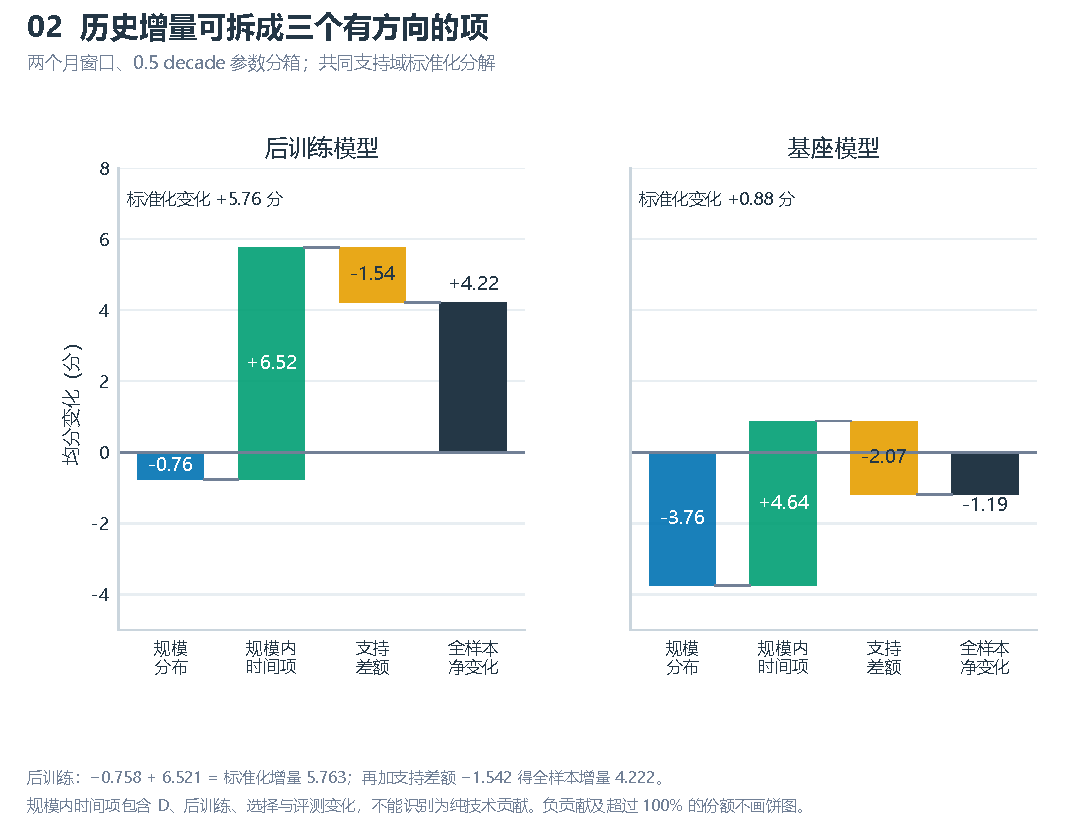
\includegraphics[width=0.84\linewidth]{figures/Q4/02_contributions.pdf}
 \caption{两类模型历史能力增量的参数分布、同格变化及支持差}
 \label{fig:q4-contributions}
\end{figure}

\subsubsection{分解结果的敏感性}

改变参数格宽与样本窗口可考察分解对共同支持划分的依赖。在两月窗口下，后训练组采用 $0.25$、$0.50$、$0.75$ decade 参数格时，规模分布份额依次为 $-16.47\%$、$-13.15\%$、$-50.08\%$：在主开放口径内符号相同，幅度变化明显，见图\ref{fig:q4-decomp-sensitivity}。再以开发者为抽样块重复抽取 80 次，主格宽下参数分布项的第 5 至第 95 百分位为 $-2.329$ 至 $0.257$ 分，跨过零；同格项对应为 $4.679$ 至 $8.460$ 分。若进一步只比较相同开发者的共同参数格，后训练组两期仅保留 6 和 8 个模型，难以据此估计总体中排除开发者差异后的变化。

开放模型的筛选口径也会改变贡献分解。表\ref{tab:q4-open-sensitivity}在相同的两月窗口和 $0.5$ decade 参数格下比较三种口径。主口径与明确标注开放权重的严格口径中，参数分布项均为负；仅按宽许可证标签筛选时，该项转为正值。这说明 $-13.15\%$ 是主样本条件下的参数规模份额，不能视为所有开放筛选方式下不变的比例；相较之下，三种口径的同格变化项均为正。结合抽样结果，历史得分提高的主要数值部分来自同参数格内的变化，但其中仍混有训练数据量、后训练方式和入榜选择的影响。

\begin{table}[htbp]
 \centering\small
 \caption{开放筛选口径对后训练组贡献分解的影响（两月窗口，$0.5$ decade）}
 \label{tab:q4-open-sensitivity}
 \begin{tabular}{lrrrrr}
 \toprule
 筛选口径 & 共同支持早/晚 & 标准化变化 & 参数分布 & 同格变化 & 参数份额\\
 \midrule
 主口径 & 313/423 & 5.763 & $-0.758$ & 6.521 & $-13.15\%$\\
 明确开放权重 & 31/58 & 6.758 & $-0.362$ & 7.121 & $-5.36\%$\\
 宽许可证标签 & 184/317 & 7.236 & 0.391 & 6.845 & $5.40\%$\\
 \bottomrule
 \end{tabular}
\end{table}

\begin{figure}[htbp]
 \centering
 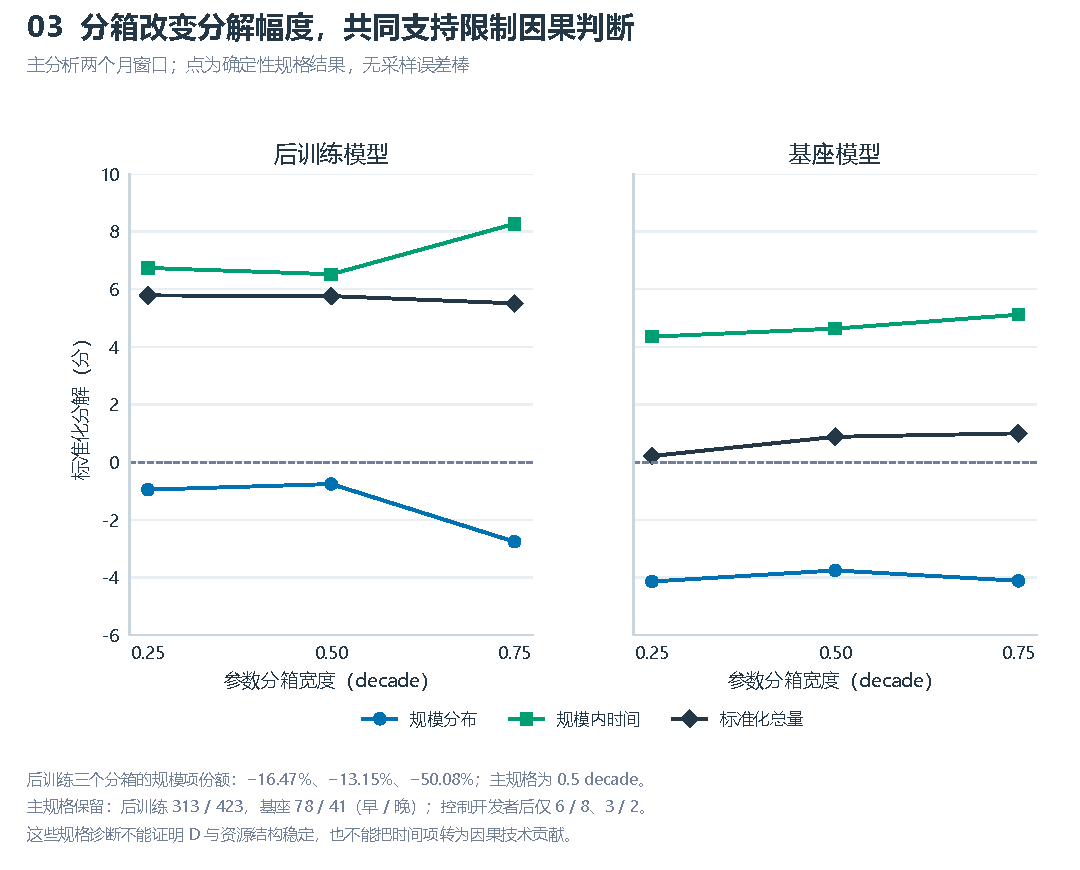
\includegraphics[width=0.84\linewidth]{figures/Q4/03_sensitivity.pdf}
 \caption{参数格宽度变化下的规模分布与同格变化}
 \label{fig:q4-decomp-sensitivity}
\end{figure}

\subsection{算力放缓下的能力前沿}

\subsubsection{预测对象与模型比较}

为描述高分模型群的典型上沿，令 $F_t$ 为同类型模型在截至 $t$ 的最近两个自然月中，式\eqref{eq:q4-score}的第 90 百分位。采用两个月窗口可以降低单个极端记录的影响，同时保留近期变化。观测截点处，后训练组 $F_0=40.445$ 分，基础预训练组为 21.032 分。本文对二者分别预测，并在下一节单独处理“截至目标日的累计最高分”。

设 $z_i=\operatorname{logit}(S_i/100)$，$t_i$ 为距统一基日的月数；对恰为 0 或 100 分的边界值，先将得分比例限制在 $[0.001,0.999]$ 内。分别建立常数基线、两月前沿趋势、均值资源模型，以及以 $\tau=0.9$ 为目标的分位资源模型\cite{koenker2017}。最后一种模型求解
\begin{equation}
 \min_{a,b_N,b_t}\sum_i\rho_{0.9}
 \left[z_i-a-b_N\log_{10}N_i-b_tt_i\right],\qquad
 \rho_\tau(u)=u\{\tau-\mathbf1(u<0)\},
 \label{eq:q4-quantile-fit}
\end{equation}
并采用线性规划得到系数。均值资源模型使用相同解释变量拟合均值关系，两月趋势仅利用历史 $F_t$ 的时间轨迹。四个候选都以未来两个完整自然月的 $F_t$ 为比较目标：每一轮仅用测试窗口开始前的提交版本和当时可见的 C4 资源记录拟合，再计算测试窗口误差\cite{forecasting2021}。

表\ref{tab:q4-backtest}与图\ref{fig:q4-backtests}给出四个滚动窗口的结果。后训练组分位资源模型 RMSE 为 2.199 分，略低于均值资源模型的 2.237；基础组则以常数模型的 7.633 分最低。全部候选的测试 $R^2$ 均为负值，四个窗口还存在重叠，因此该比较用于选择情景模型及观察误差，不据此推定长期预测精度。

\begin{table}[htbp]
 \centering\small
 \caption{最近两月能力前沿的四窗口滚动预测 RMSE（分）}
 \label{tab:q4-backtest}
 \begin{tabular}{lrrrr}
 \toprule
 类型 & 常数 & 两月趋势 & 均值资源 & 分位资源\\
 \midrule
 后训练 & 3.737 & 3.053 & 2.237 & 2.199\\
 基础预训练 & 7.633 & 9.571 & 9.763 & 10.561\\
 \bottomrule
 \end{tabular}
\end{table}

\begin{figure}[htbp]
 \centering
 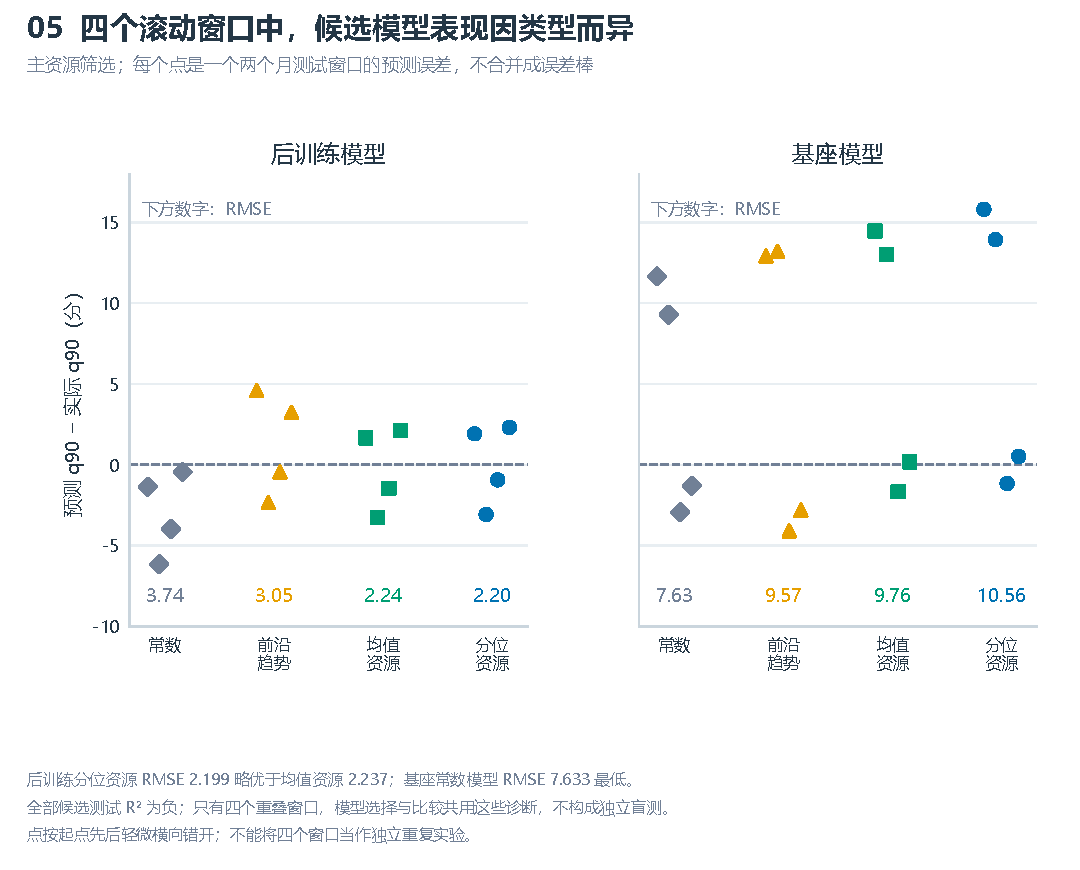
\includegraphics[width=0.85\linewidth]{figures/Q4/05_backtests.pdf}
 \caption{两类模型的最近两月能力前沿滚动预测误差}
 \label{fig:q4-backtests}
\end{figure}

\subsubsection{资源配置情景与前沿预测}

后训练组采用分位资源模型作为主情景。设 $g_C$ 为 C4 的年算力对数增长率，$s$ 为未来增长倍率；取 $s=1,1/2,1/4,0$ 分别表示沿历史速率、增速减半、增速降至四分之一和停止增长。令 $\eta=0.5$ 表示新增资源的一半按十进对数分配给参数量，其余对应训练量；令 $\lambda=0.5$ 为未来时间项的保留系数。以当前两月 $F_0$ 为锚，预测式为
\begin{equation}
 \widehat F(H;s)=100\,\sigma\!\left[
 \operatorname{logit}(F_0/100)
 +b_N\eta s g_C\frac{H}{12}
 +\lambda b_tH\right],\qquad
 \sigma(x)=\frac{1}{1+e^{-x}}.
 \label{eq:q4-frontier-forecast}
\end{equation}
其中 $H$ 为距观测截点的月份。C2 未提供逐模型训练量，故 $\eta$ 是资源分配情景而非由能力数据单独估计的参数。算力增速减半指年对数速率由 0.6903 降至约 0.3452，年倍率由 4.901 降至约 2.214。

后训练组的最后观测日为 2025 年 3 月 13 日。按增速减半，2026 年 3 月 13 日的 12 个月 $F$ 预测为 53.828 分，2027 年 3 月 13 日的 24 个月预测为 66.681 分；其余增长情景列于表\ref{tab:q4-growth}。将 C4 资源核对范围由主口径放宽后，后训练组分位资源模型的四窗 RMSE 为 2.195 分，增速减半时的 12、24 个月预测为 53.222 和 65.591 分，与主口径接近。基础组最后观测日为 2025 年 3 月 9 日，短期比较选择了常数模型，对应的两月第 90 百分位参考值为 21.032 分。图\ref{fig:q4-forecasts}并列显示两类模型的预测。所列日期均从附件观测截点起算。

\begin{table}[htbp]
 \centering\small
 \caption{后训练模型在不同算力增长情景下的两月第 90 百分位预测（分）}
 \label{tab:q4-growth}
 \begin{tabular}{lrrrr}
 \toprule
 预测期限 & 停止增长 & 历史增速的四分之一 & 历史增速减半 & 保持历史增速\\
 \midrule
 12 个月 & 49.157 & 51.496 & 53.828 & 58.432\\
 24 个月 & 57.921 & 62.403 & 66.681 & 74.422\\
 \bottomrule
 \end{tabular}
\end{table}

\begin{figure}[htbp]
 \centering
 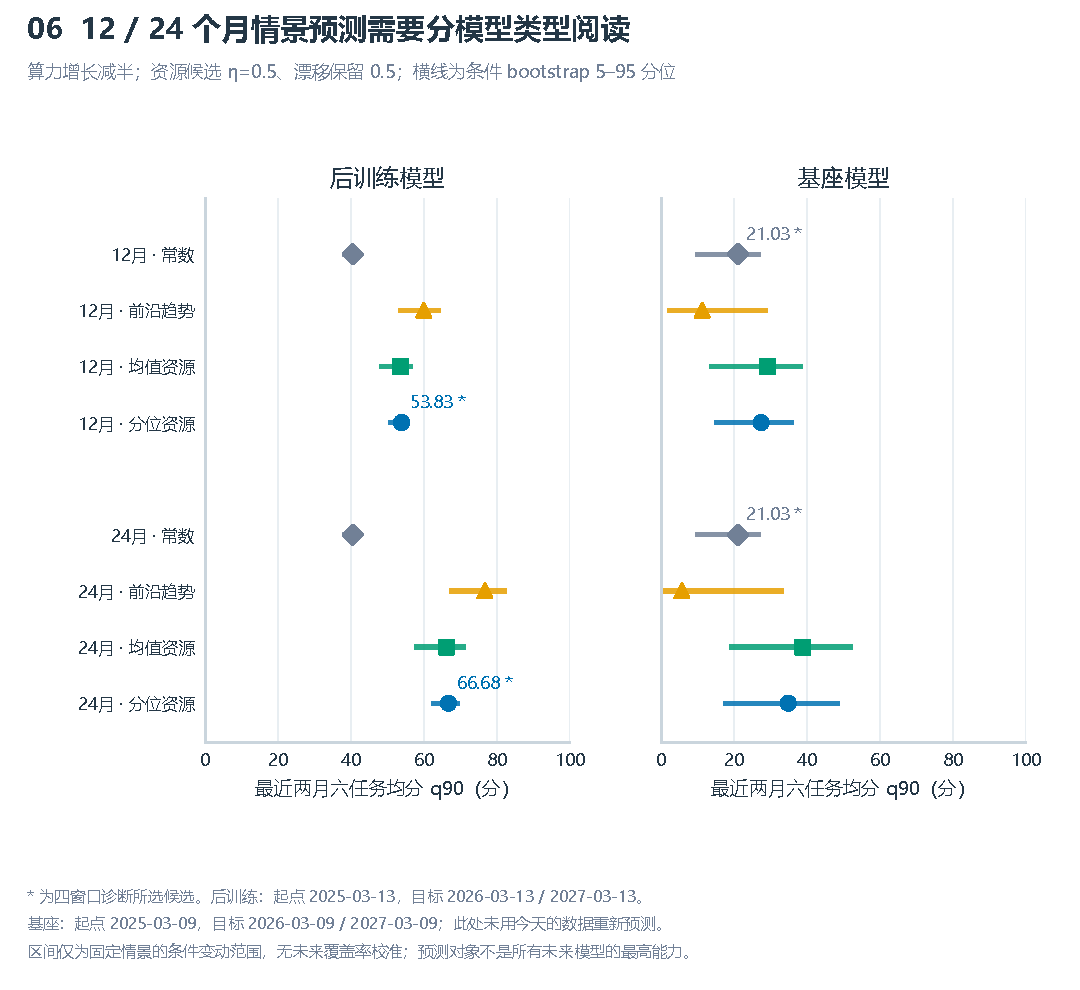
\includegraphics[width=0.86\linewidth]{figures/Q4/06_forecasts.pdf}
 \caption{算力增速减半时两类模型的 12 个月与 24 个月前沿情景}
 \label{fig:q4-forecasts}
\end{figure}

\subsubsection{预测范围与外推程度}

为区分参数扰动和建模情景，先按开发者为单位重复抽取 80 次，在固定增速减半、资源分配及时间保留系数下重新估计，得到后训练组 12 个月的第 5 至第 95 百分位范围 $50.302$--$56.007$ 分，24 个月为 $61.983$--$69.805$ 分。随后改变候选模型、资源筛选、增长速率、$\eta$、$\lambda$、近期窗口及分位水平，取各情景条件范围的并集；最后将四窗口最大绝对误差作为固定偏差压力叠加。表\ref{tab:q4-uncertainty}与图\ref{fig:q4-uncertainty}显示三层范围逐步扩大。它们分别回答“固定参数下怎样波动”“合理情景改变后差多少”“若延续已见偏差会怎样”，尚未用未来观测校准覆盖率。

\begin{table}[htbp]
 \centering\small
 \caption{后训练模型、算力增速减半下的三层条件范围（分）}
 \label{tab:q4-uncertainty}
 \begin{tabular}{lrrr}
 \toprule
 期限 & 固定情景块抽样 & 多情景条件并集 & 叠加固定偏差压力\\
 \midrule
 12 个月 & 50.302--56.007 & 37.755--72.236 & 31.590--78.400\\
 24 个月 & 61.983--69.805 & 37.755--90.640 & 31.590--96.805\\
 \bottomrule
 \end{tabular}
\end{table}

\begin{figure}[htbp]
 \centering
 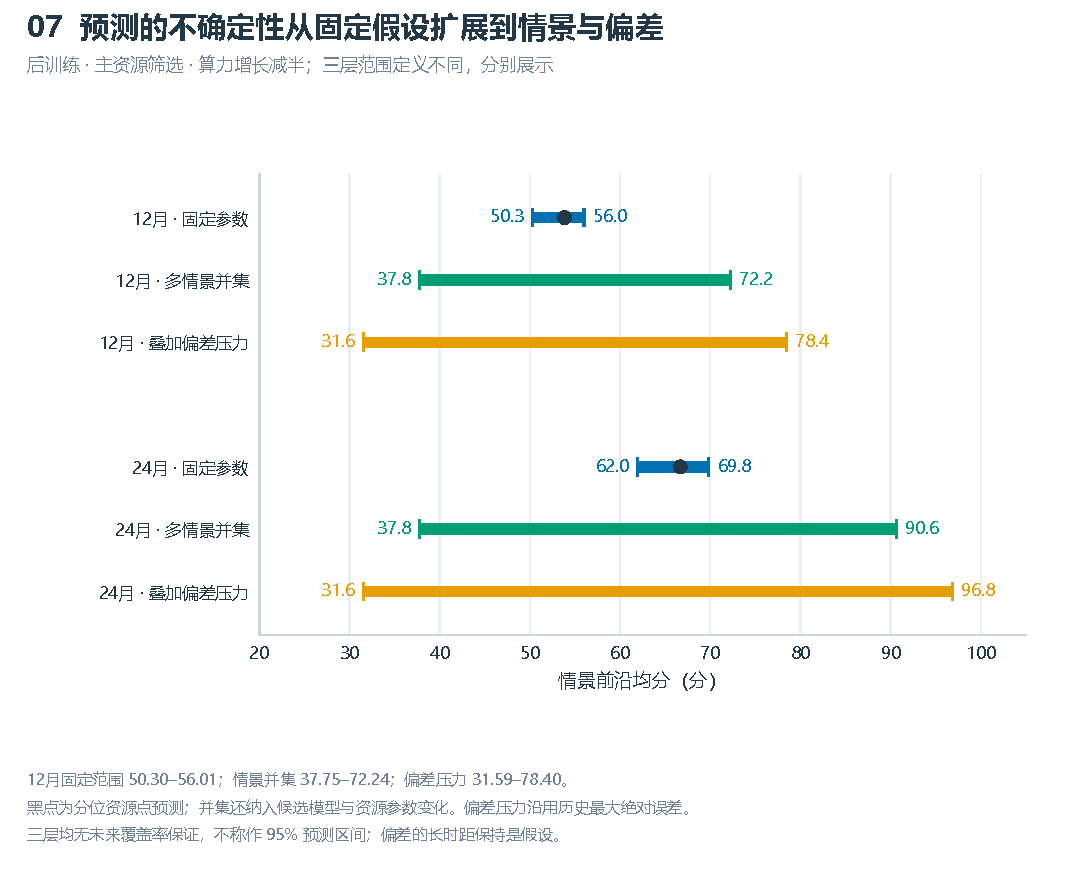
\includegraphics[width=0.85\linewidth]{figures/Q4/07_uncertainty.pdf}
 \caption{固定情景、多情景与偏差压力下的能力前沿范围}
 \label{fig:q4-uncertainty}
\end{figure}

24 个月预测期限约为后训练组已观测时间跨度的 2.64 倍，因此表中长期范围随模型和情景变化显著扩大。近期第 90 百分位描述的是高分模型群，并不直接回答“截至未来目标日的最高分”，下节另建立最高能力边界。

\subsection{截至目标日的最高能力边界}

令 $R_t=\max_{i:d_i\leq t}S_i$ 表示截止日期 $t$ 以前，同一开放筛选和模型类型下所有已提交版本的累计最高分。它至少保持已达到的历史纪录。以纪录保持作为基线，并在式\eqref{eq:q4-frontier-forecast}的第 90 百分位预测之上，加入近期最高分相对第 90 百分位的差额，构造另一种条件上尾情景：
\begin{equation}
 \widehat R^{\rm base}_{t+H}=R_t,\qquad
 \widehat R^{\rm tail}_{t+H}(w)=
 \min\!\left\{100,\max\left[R_t,
 \widehat F(H)+\Delta_{\rm tail}(w)\right]\right\},
 \label{eq:q4-maximum}
\end{equation}
其中 $\Delta_{\rm tail}(w)$ 是最近 $w$ 个月样本最高分与同期第 90 百分位之差，主情景用 $w=2$，并以 1、3 个月比较尾差变化。两项分别表示“不刷新纪录”的经验基线和“近期上尾差额继续存在”的条件方案。

四个重叠的两月回测窗口均未刷新此前累计纪录，故纪录保持基线在这些窗口的 RMSE 为 0；后训练组 1、2、3 月尾差方案的 RMSE 分别为 3.376、2.254、3.683 分。这一短期结果支持将纪录保持作为基线，同时保留上尾情景考察未来可能的纪录更新。算力增速减半时，后训练组当前累计最高分为 51.231，12、24 个月的条件最高边界分别为 60.600 和 73.453 分；将尾差窗口改为 1 或 3 个月，相应范围分别为 60.474--61.203 与 73.327--74.057 分。基础预训练组当前累计最高分 38.441，在其常数前沿情景下两期均保持该值，见表\ref{tab:q4-maximum}和图\ref{fig:q4-maximum}。这些范围反映尾差取法的变化，而非预测误差的概率区间。

\begin{table}[htbp]
 \centering\small
 \caption{算力增速减半时的近期高分群与累计最高能力（分）}
 \label{tab:q4-maximum}
 \begin{tabular}{lrrrrr}
 \toprule
 类型 & 当前纪录 & 12 月 $F$ & 12 月条件最高 & 24 月 $F$ & 24 月条件最高\\
 \midrule
 后训练 & 51.231 & 53.828 & 60.600 & 66.681 & 73.453\\
 基础预训练 & 38.441 & 21.032 & 38.441 & 21.032 & 38.441\\
 \bottomrule
 \end{tabular}
\end{table}

\begin{figure}[htbp]
 \centering
 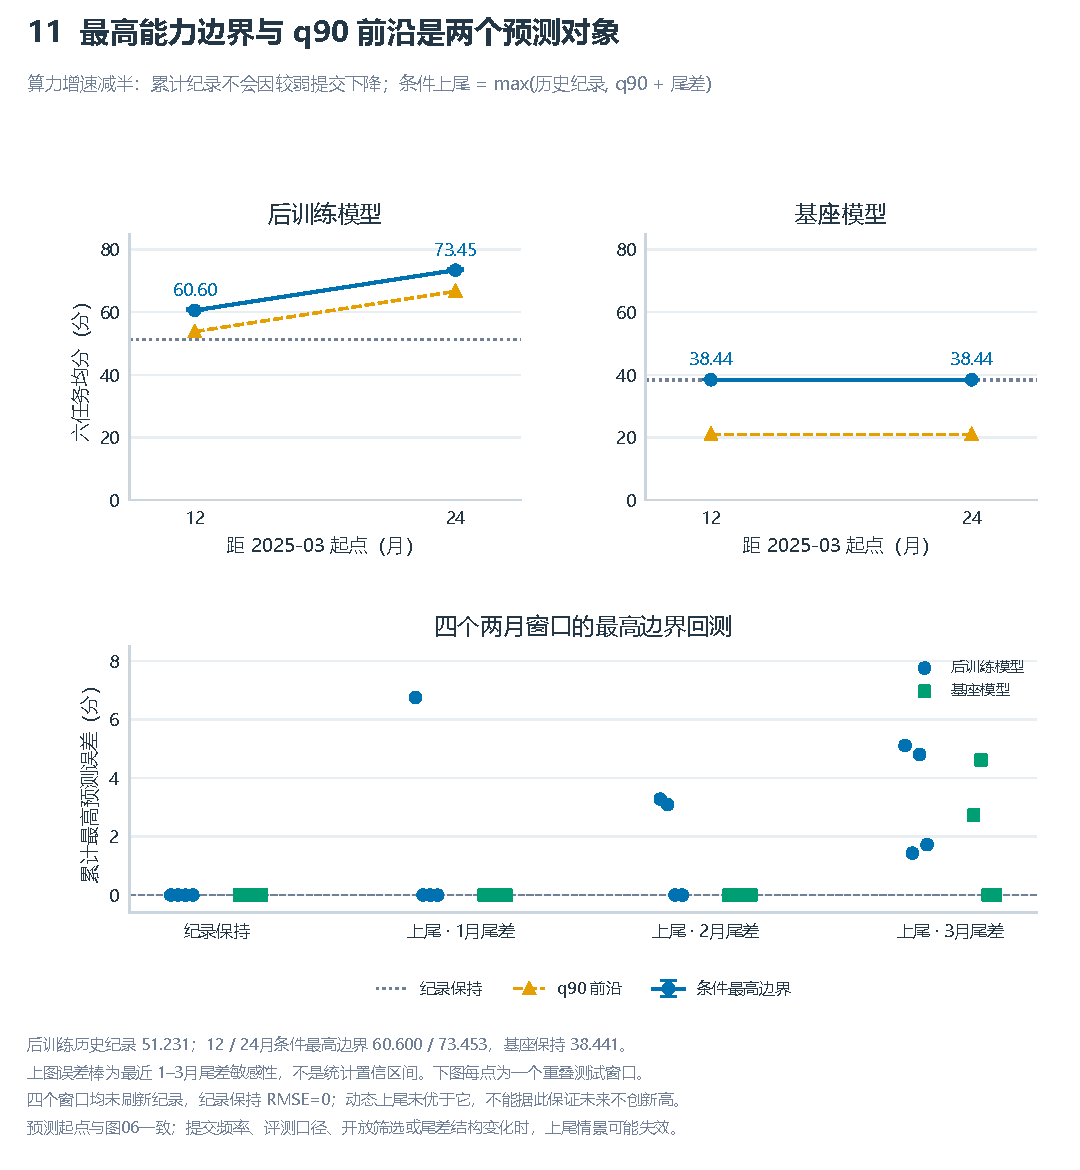
\includegraphics[width=0.85\linewidth]{figures/Q4/11_maximum_boundary.pdf}
 \caption{最近两月高分群、纪录保持基线和条件最高能力边界}
 \label{fig:q4-maximum}
\end{figure}

\subsection{Loss 与能力得分的连接}

\subsubsection{来源内单调映射及检验}

C6 的 Loss 来自不同模型、验证语料和训练阶段。将来源及 Loss 类型分别保留，在每个具有足够成对记录的来源 $s$ 内建立有界的单调关系
\begin{equation}
 \operatorname{logit}\!\left(\frac{S}{100}\right)
 =a_s+b_s\ell_s,\qquad b_s\leq0,
 \label{eq:q4-bridge}
\end{equation}
其中 $\ell_s$ 为该来源记录的 Loss。若估计斜率不满足 Loss 降低、能力提高的方向，模型退回来源内常数关系。对来源内每条记录依次留出、重拟合并预测，同时与常数关系比较。表\ref{tab:q4-bridge-validation}及图\ref{fig:q4-bridge-validation}给出具有 validation 标签的三个主要来源。Qwen2 和 Qwen2.5 的单调关系优于各自常数对照；Pythia 虽具有较高的来源可比性，其小样本关系在留一预测中反而略差。附件的 validation 标签用于区分数据口径，尚不足以建立与第三问 Loss 的直接数值等价。

\begin{table}[htbp]
 \centering\small
 \caption{C6 同来源 Loss--能力映射的逐点留出 RMSE（分）}
 \label{tab:q4-bridge-validation}
 \begin{tabular}{lrrr}
 \toprule
 来源 & 样本数 & 单调关系 & 来源内常数\\
 \midrule
 Pythia validation & 7 & 0.538 & 0.426\\
 Qwen2 validation & 4 & 7.048 & 10.708\\
 Qwen2.5 validation & 6 & 2.655 & 15.074\\
 \bottomrule
 \end{tabular}
\end{table}

\begin{figure}[htbp]
 \centering
 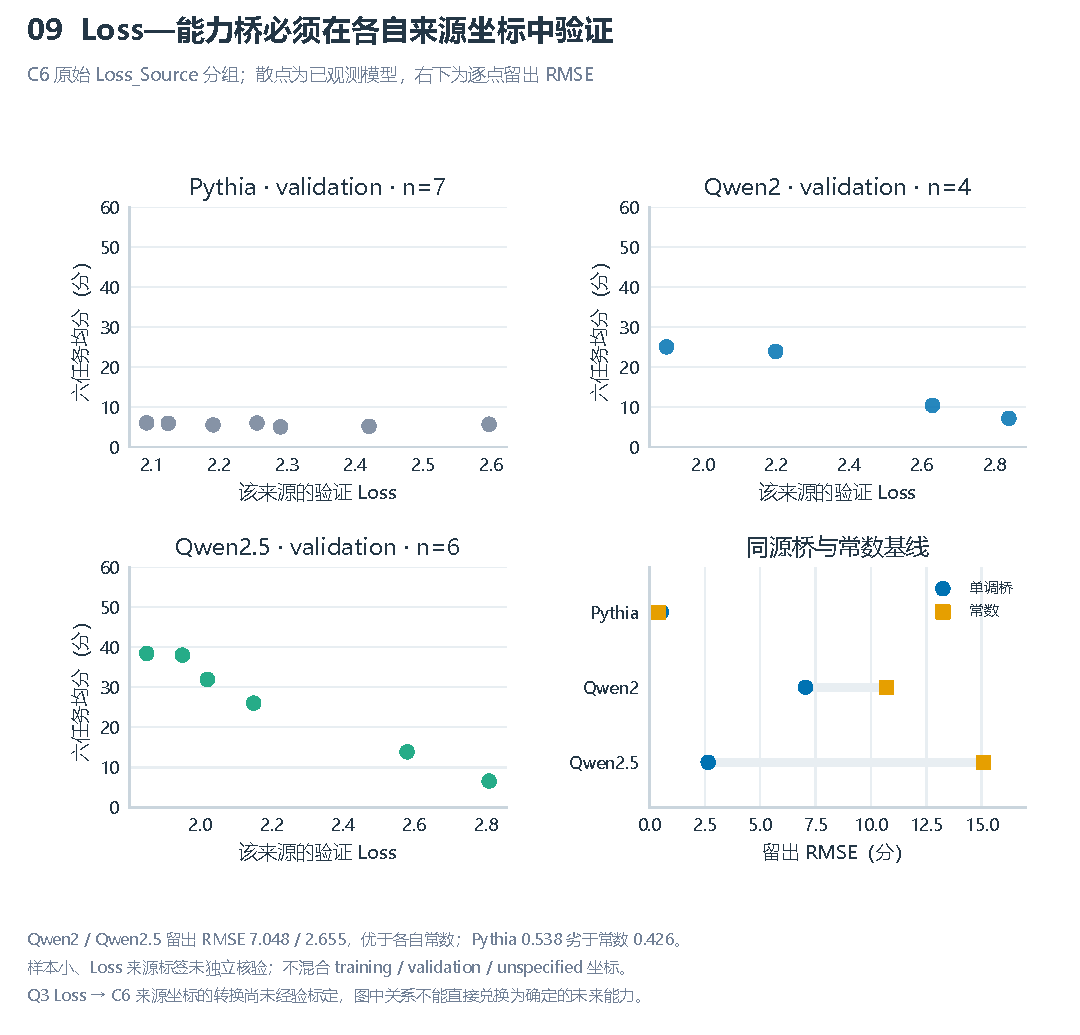
\includegraphics[width=0.85\linewidth]{figures/Q4/09_bridge_validation.pdf}
 \caption{C6 各来源的 Loss--能力关系及逐点留出误差}
 \label{fig:q4-bridge-validation}
\end{figure}

\subsubsection{第三问配置的条件能力换算}

第三问输出的 Loss 与 C6 各来源的 Loss 尚无成对标定。为考察数值换算对这一差异的敏感程度，分别给出正尺度、偏移及上游预测扰动情景
\begin{equation}
 \ell_s=a\{\widehat L_{\rm Q3}+\delta\}+b,
 \quad a\in\{0.9,1,1.1\},\quad
 b\in\{-0.1,0,0.1\},\quad
 \delta\in\{-0.05,0,0.05\}.
 \label{eq:q4-coordinate}
\end{equation}
仅当 $N$ 及变换后的 $\ell_s$ 都位于该来源的观测范围，才代入式\eqref{eq:q4-bridge}。对第三问固定配方、已观测配方联立和独立质量三类配置，分别在五种可拟合的 C6 来源内施加 27 组坐标与上游 Loss 变化。这些区间反映连接假设改变后的结果范围。

以 8192 Token、幂函数质量成本、$10^{22}$ FLOPs 下第三问选择的配方 172 为例，其预测 Loss 为 2.094421。表\ref{tab:q4-bridge-stress}和图\ref{fig:q4-bridge-stress}展示 Qwen2 与 Qwen2.5 两个来源内有观测支持的换算。取 $a=1,b=\delta=0$，预测得分分别为 22.371 与 28.695；改变坐标假设后，前者在 22/27 个可换算情景中为 13.601--27.462，后者在 23/27 个情景中为 15.057--39.197。与相同 $N$ 的规模主干模型相比，模型内得分差在这些可换算情景中保持正值，但其幅度与来源内留出误差处于相近量级，尚需同坐标实验辨别真实改善。

\begin{table}[htbp]
 \centering\small
 \caption{$10^{22}$ FLOPs 下配方 172 的条件得分与坐标变化范围（分）}
 \label{tab:q4-bridge-stress}
 \begin{tabular}{lrrrr}
 \toprule
 C6 来源 & 可换算格 & 名义得分 & 得分范围 & 对规模主干的得分差\\
 \midrule
 Qwen2 validation & 22/27 & 22.371 & 13.601--27.462 & 0.322--3.596\\
 Qwen2.5 validation & 23/27 & 28.695 & 15.057--39.197 & 0.473--5.734\\
 \bottomrule
 \end{tabular}
\end{table}

\begin{figure}[htbp]
 \centering
 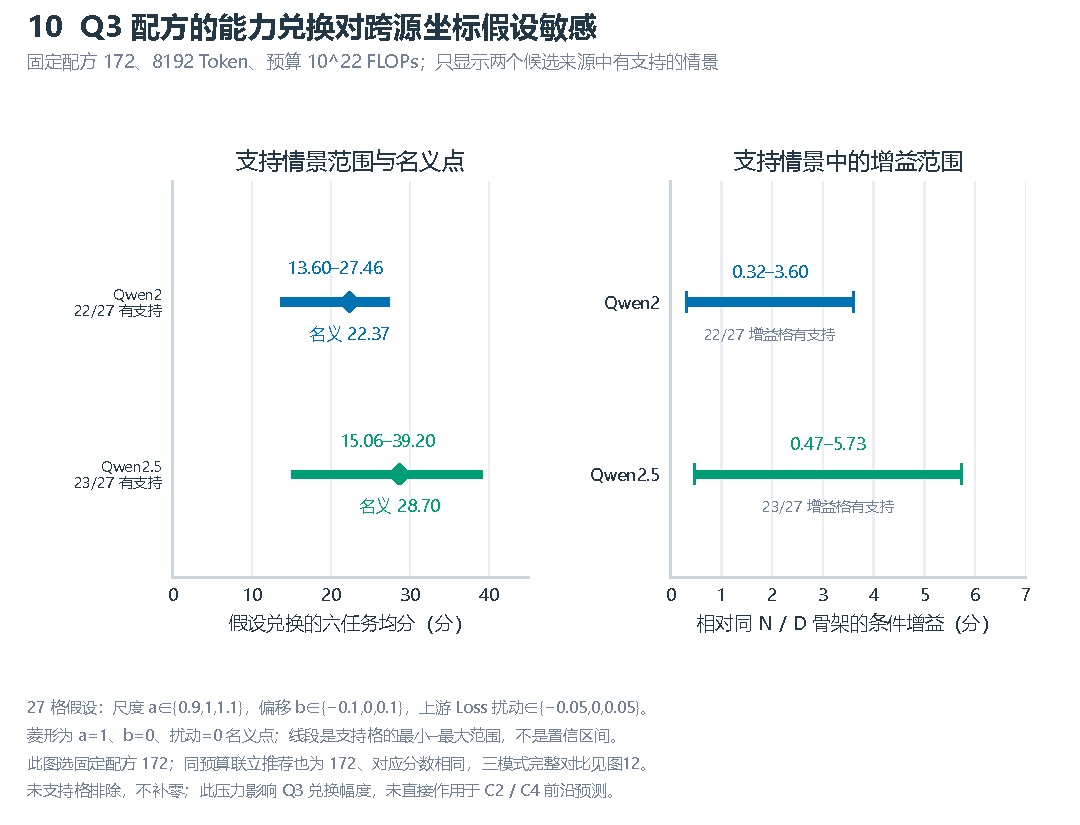
\includegraphics[width=0.85\linewidth]{figures/Q4/10_bridge_stress.pdf}
 \caption{配方 172 在不同 Loss 坐标假设下的能力得分与增量}
 \label{fig:q4-bridge-stress}
\end{figure}

图\ref{fig:q4-policy-bridge}进一步把第三问的三种投入方式放在相同来源坐标情景中比较。$10^{19}$ FLOPs 下固定配方 172 在部分成本设置中不可行；8192 Token、幂成本下联立配方 477 的 $N=0.0873$ 十亿，独立质量方案的 $N=0.1309$ 十亿，均低于 Qwen2 与 Qwen2.5 来源中的最小参数量，故该预算没有相应得分。到 $10^{22}$ 和 $10^{24}$ FLOPs，固定配方与联立配置均选择配方 172，二者在相同情景下得分重合。独立质量方案在 $10^{22}$ FLOPs 下的名义得分为 Qwen2 的 24.489 和 Qwen2.5 的 32.081 分；它改变了质量输入机制，数值差异应与这一前提同时阅读。扩展到全部配方、成本与来源组合时，部分方案相对规模主干的增量在坐标变化中改变符号，方案间排序也会改变。因此，第三问方案的得分比较须与来源和坐标假设一同给出；直接由 C2/C4 拟合的能力前沿式\eqref{eq:q4-frontier-forecast}则不涉及这一换算。

\begin{center}
 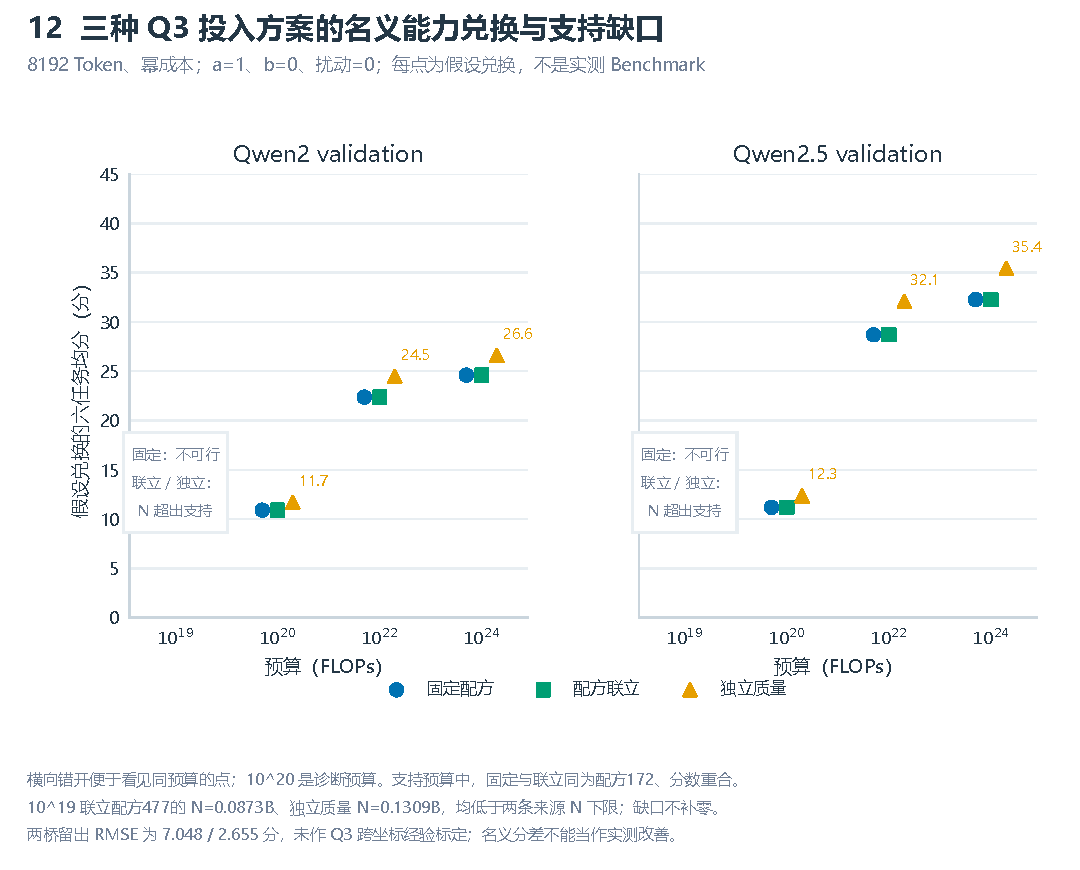
\includegraphics[width=0.80\linewidth]{figures/Q4/12_policy_bridge.pdf}
 \captionof{figure}{三种第三问资源配置在两种 C6 来源中的条件得分}
 \label{fig:q4-policy-bridge}
\end{center}

\subsection{本问输出与结果讨论}

表\ref{tab:q4-output}汇总历史分解、情景预测与第三问方案换算，并注明各结果的使用条件。

\begin{table}[htbp]
 \centering\small
 \caption{问题四的主要结果及跨问题使用方式}
 \label{tab:q4-output}
 \begin{tabular}{p{2.5cm}p{4.2cm}p{5.8cm}}
 \toprule
 结果 & 数值或模型 & 使用方式\\
 \midrule
 历史能力分解 & 后训练组参数分布 $-0.758$ 分，同格变化 6.521 分 & 描述共同支持样本的变化；开放筛选改变时须重新计算\\
 近期高分群 & 增速减半时 12/24 月第 90 百分位 53.828/66.681 分 & 作为后训练模型资源情景下的能力预测\\
 累计最高能力 & 纪录保持 51.231 分；条件上尾 60.600/73.453 分 & 分别提供已达到的基线和未来刷新纪录的情景\\
 Loss--能力联系 & C6 来源内单调映射及逐点留出误差 & 先核对来源与参数、Loss 范围，再比较第三问配置\\
 配方换算 & 配方 172 的两来源名义得分 22.371/28.695 分 & 仅在明示 Loss 坐标假设下讨论方案得分与排序\\
 \bottomrule
 \end{tabular}
\end{table}

综上，参数格标准化分解刻画了历史能力增长中的规模分布与同格变化；资源情景模型分别给出近期高分群和累计最高能力的未来参考值。来源内 Loss--能力关系进一步连接了第三问的训练配置，配方得分随 Loss 坐标假设而变化。上述结果为分析开源模型能力演进及不同算力路径下的训练方案提供了定量依据。



\section{模型评价}

本文的质量评价、配比预测、广义标度律和预算优化依次衔接，使训练数据选择与资源投入能够放在同一 Loss 目标下比较。质量评分通过扩展样本对照检验，二阶配比模型通过交叉验证及不同规模实验组比较；标度律利用训练轨迹和跨模型族下降方向检验，预算解则通过假设敏感性与公开模型的规模排序进行分析。能力预测同时报告近期高分群与累计最高分，避免两种目标混用。

模型的数值解释随数据范围而变化。质量项来自半合成记录，第一问质量评分与第二问 Loss 的连接采用尺度映射；配比模型在个别连续方案中出现负预测 Loss，需在应用时收紧其范围。最高预算的资源配置达到已有数据上界，长期能力预测则依赖资源增长与近期尾差情景。今后若获得同一训练系统下的质量、配比、Loss 与 Benchmark 成对实验，可进一步校准跨问题连接并检验更大规模的配置。

\bibliographystyle{gmcm}
\bibliography{reference}
\end{document}
